\documentclass[10pt, a4paper]{article}
\usepackage[vmargin=1in,hmargin=1in]{geometry}
\usepackage[pdftex]{graphicx}
\usepackage{amsmath,amssymb}
\usepackage[utf8x]{inputenc}
\usepackage[english]{babel}
\usepackage[pdftex]{graphicx}
\usepackage{ctable}
\usepackage{appendix}
\usepackage{verbatim,listings}
\usepackage{epstopdf}
\usepackage{rotating}
\usepackage[lined, boxed]{algorithm2e}
\usepackage[T1]{fontenc}
\renewcommand{\familydefault}{\sfdefault}
\newcommand{\imsize}{}
\newlength{\widthtmp}
\newcommand{\getWidth}[1]{%
  \settowidth{\widthtmp}{#1}%
  \the\widthtmp%
}
%\providecommand{\abs}[1]{\left\lvert#1\right\rvert}

\usepackage[pdftex,
pdftitle={Antidiffusion techniques to refine the numerical solution of the advection equation. Case study: Smolarkiewicz' iterative approach},
pdfauthor={G. Burger. J. Wolterink},
pdfstartview=FitH
]{hyperref}


\author{Gerhard Burger \and Jelmer Wolterink}
\title{Anti-diffusion techniques to refine the numerical solution of the advection equation\\ Case study: Smolarkiewicz' iterative approach}

\newcommand{\abs}[1]{\left\lvert#1\right\rvert}

\begin{document}
\maketitle

\section{Introduction}
The advection equation describes the transport of a substance by a fluid, due to the fluid's motion in a particular direction. It plays an important role in climate modeling, e.g. in the modeling of
\begin{itemize}
   \item Transport of trace gasses air due to wind
   \item Transport of heat by ocean water due to currents
   \item Transport of ice by ocean water due to currents
   \item Transport of warm and moist air over a colder surface by air due to wind: advection fog
\end{itemize}

A well known example of a large scale process where advection plays a role is the Thermohaline Circulation (THC). The THC advects salty water northwards in the Atlantic.

If the advection equation is solved numerically the space is discretized and this can cause diffusion. Several anti-diffusion techniques have been explored to correct for this implicit diffusion. On technique that is still in use today, be it in a generalized form, is the iterative approach developed by Smolarkiewicz in 1983 \cite{smolarki}. This approach is conceptually simple, and straightforward to implement.

In this report we will discuss the implementation of Smolarkiewicz' iterative approach in Fortran. First we will give some general remarks about numerically solving the advection equation and using anti-diffusion techniques, after that we will discuss the actual implementation and finally we will discuss some numerical results and give a short overview of the current developments in anti-diffusion techniques.

\section{Solving the advection equation}
\label{sec:solvadveq}
The continuity equation describing the advection of a non-diffusive quantity in a flow field is defined as

\begin{equation}
\frac{\partial \psi}{\partial t} + \text{ div}(V\psi) = 0
\end{equation}

where $\psi(x,y,z,t)$ is the non-diffusive scalar quantity, $V=(u,v,w)$ is the velocity vector and $x,y,z,t$ are the independent variables of space and time. In the one-dimensional case, this is

\begin{equation}
\frac{\partial \psi}{\partial t} + \frac{\partial}{\partial x}(u\psi) = 0,
\end{equation}

To solve this partial differential equation numerically we need to take into account the following constraints on the solution:

\begin{itemize}
\item Solutions should contain no unphysical overshoot or undershoot: positive definite schemes
\item Methods should be volume preserving. No loss of matter
\item The solutions should be local: the solution at any one point should not be influenced by what is going on far away from that point
\item Methods should not introduce new extrema
\end{itemize}

\subsection{Diffusion}
Figure~\ref{fig:dif} provides a nice illustration of what diffusion in 1D is. In this example the horizontal velocity $u=0.5$ is not integral, so per time step only a portion of the quantity in the grid box moves to the next grid box. The red bars show the exact solution of the advection equation

\begin{equation}
 u(x,t)=F(x-ut)=F(x-0.5t).
\end{equation}

Clearly this diffusive behavior is undesirable. If your simulation runs for some time, the solution `smears' out and becomes zero everywhere. Though the solution of this method is volume preserving and no unphysical values are introduced, it is a rather bad simulation of non-diffusive advection. Furthermore, the diffusive effect extends the domain of the substance very rapidly, which could cause interactions between the substance and substances in other domains, thereby further reducing the validity of the simulation.
\begin{figure}[htp]
\renewcommand{\imsize}{0.3\textwidth}
\begin{tabular}{ccc}
{\resizebox{\imsize}{!}{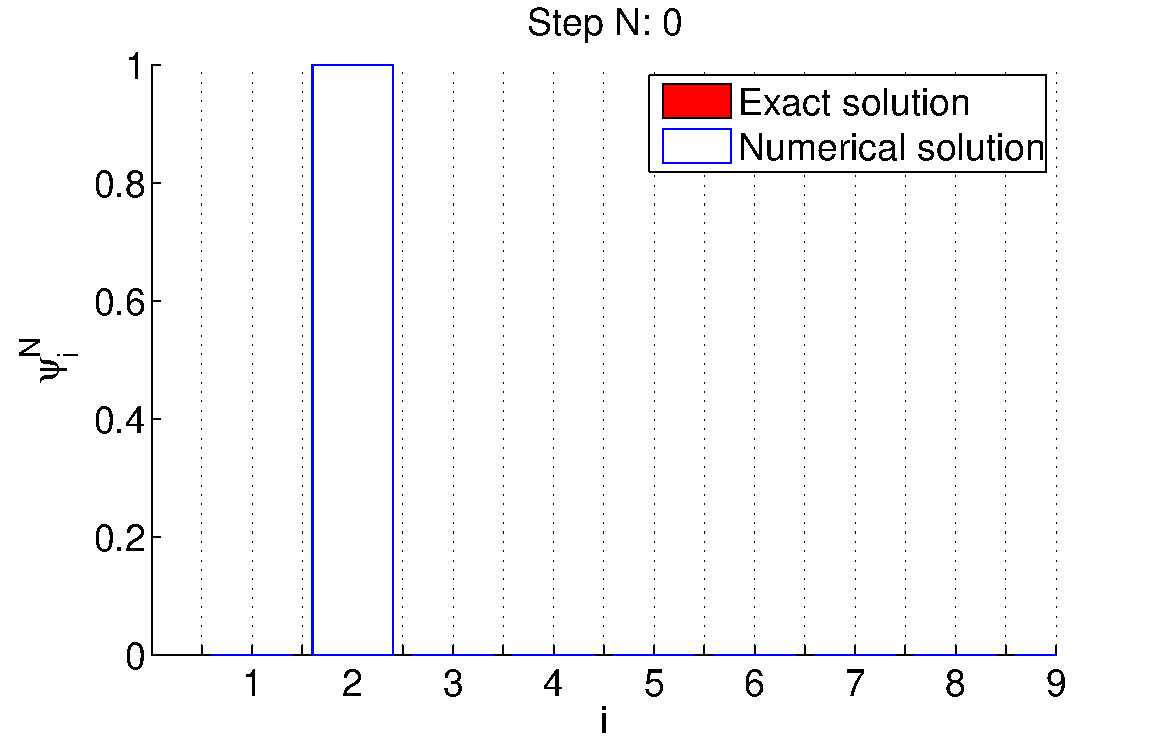
\includegraphics{../presentation/animation/anime0.pdf}}} &
{\resizebox{\imsize}{!}{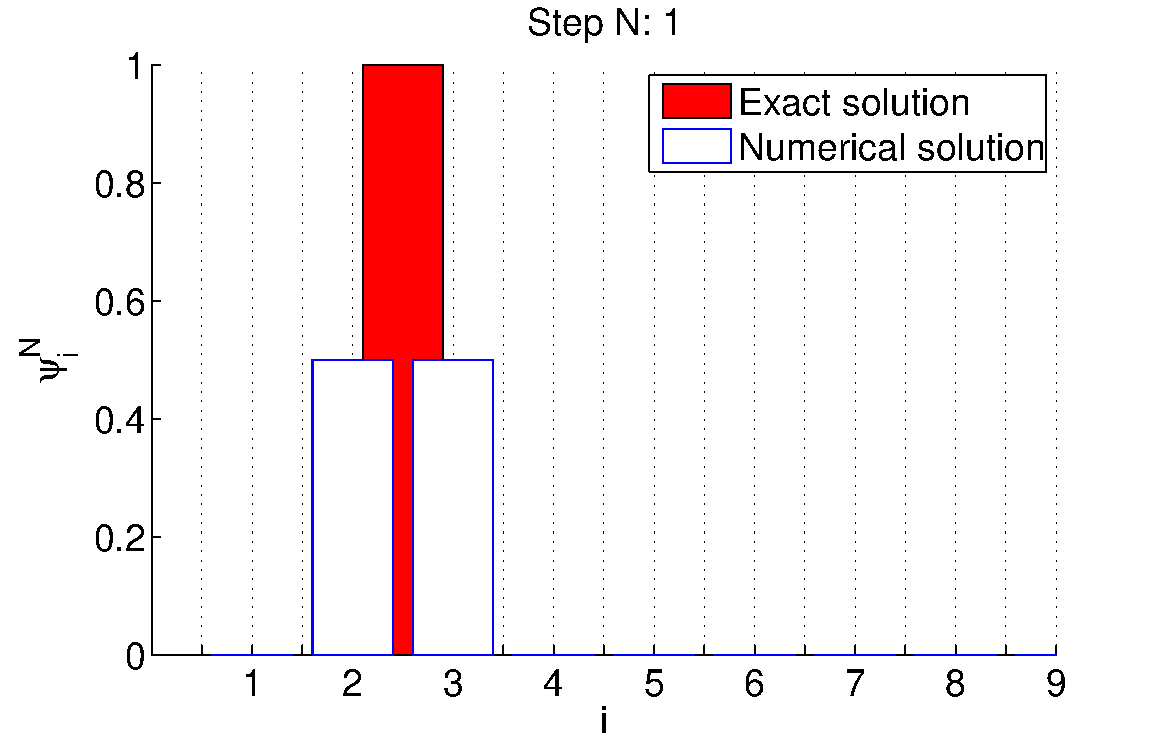
\includegraphics{../presentation/animation/anime1.pdf}}} &
{\resizebox{\imsize}{!}{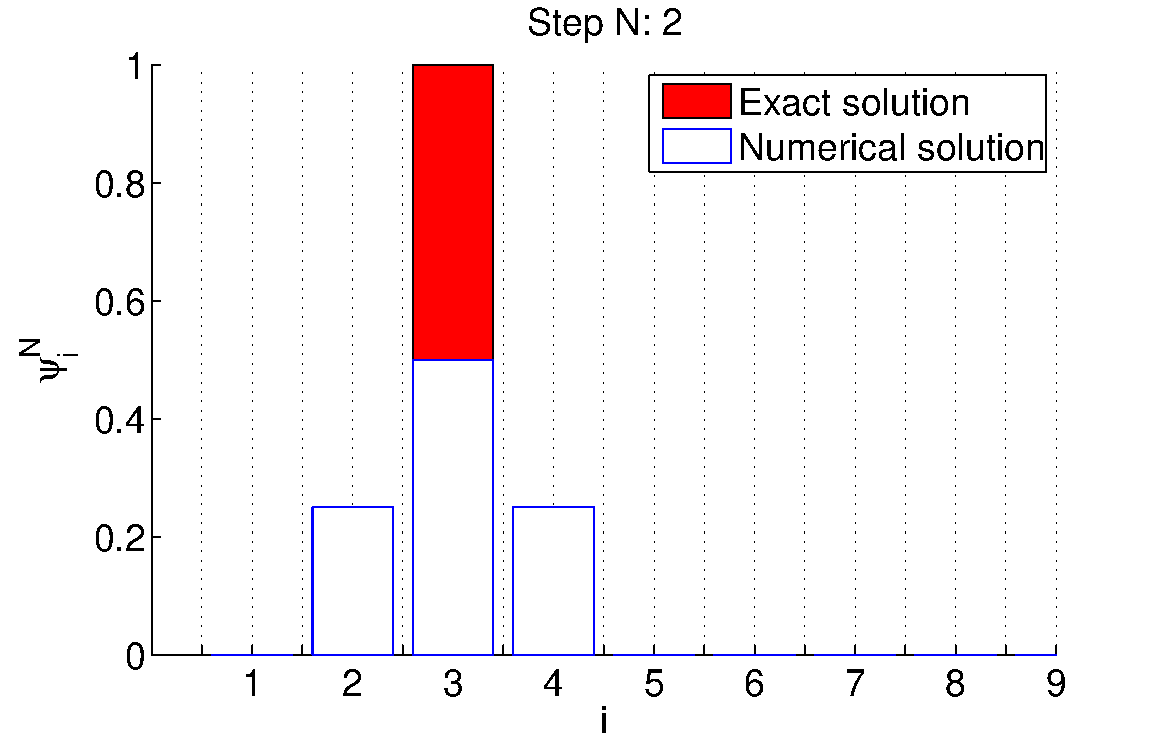
\includegraphics{../presentation/animation/anime2.pdf}}} \\
{\resizebox{\imsize}{!}{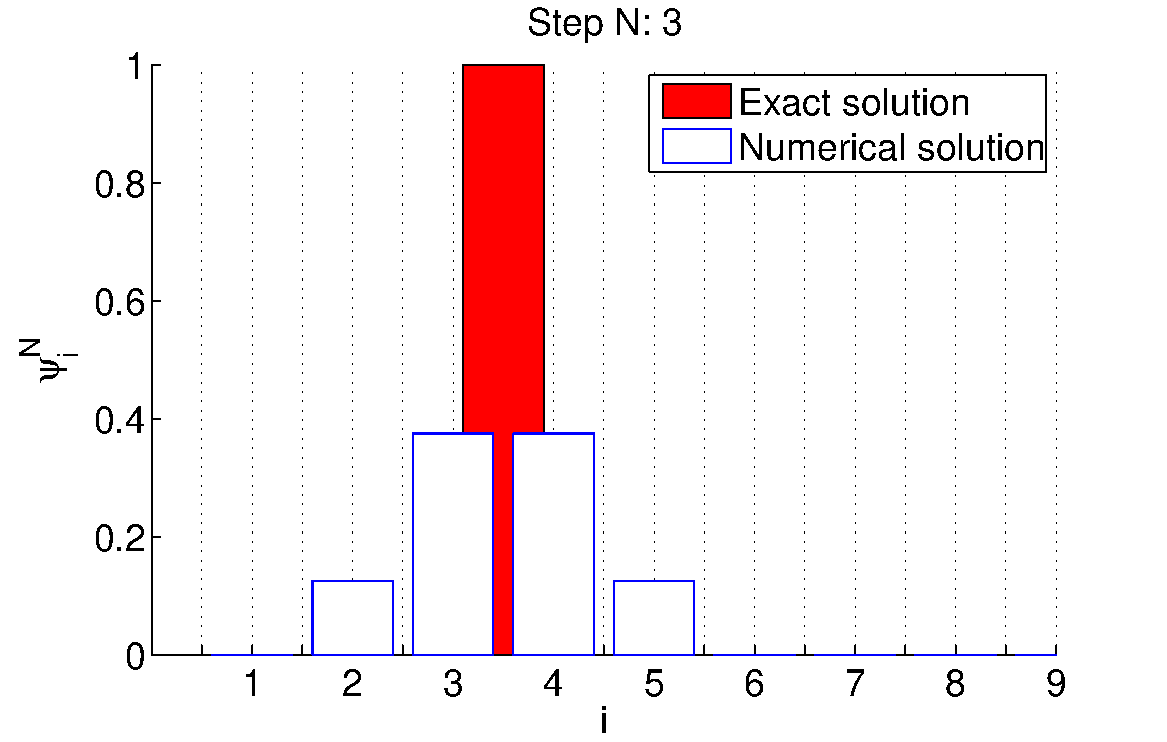
\includegraphics{../presentation/animation/anime3.pdf}}} &
{\resizebox{\imsize}{!}{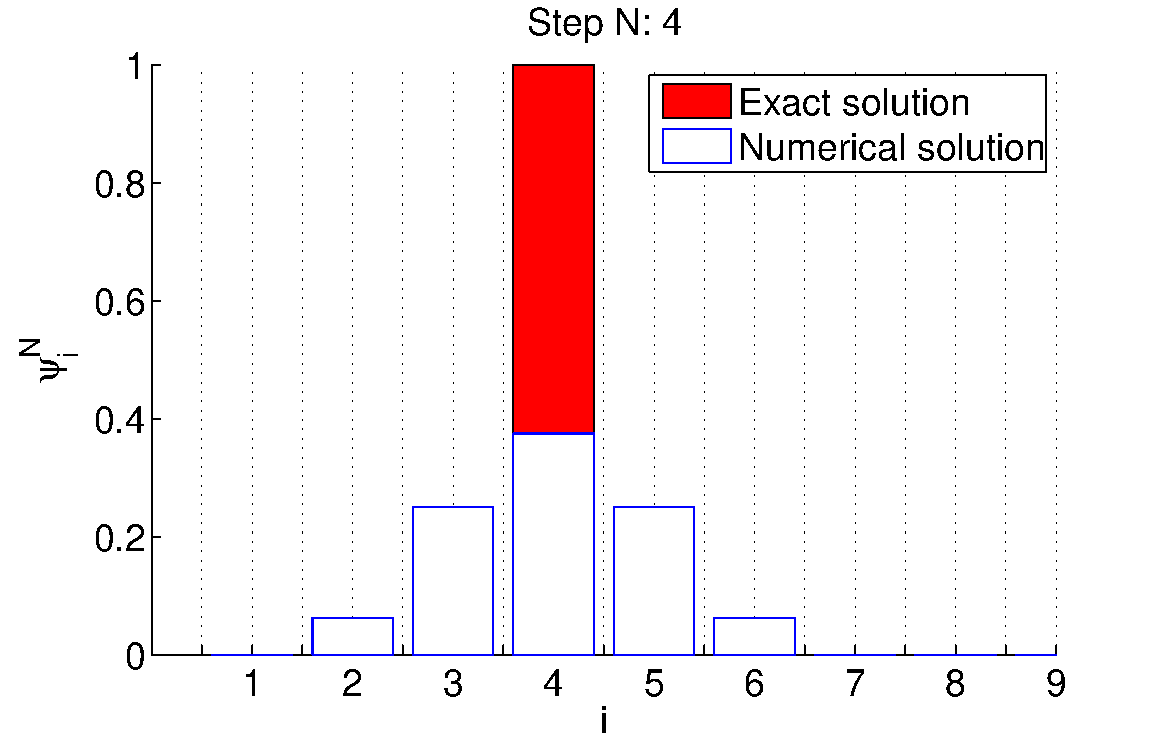
\includegraphics{../presentation/animation/anime4.pdf}}} &
{\resizebox{\imsize}{!}{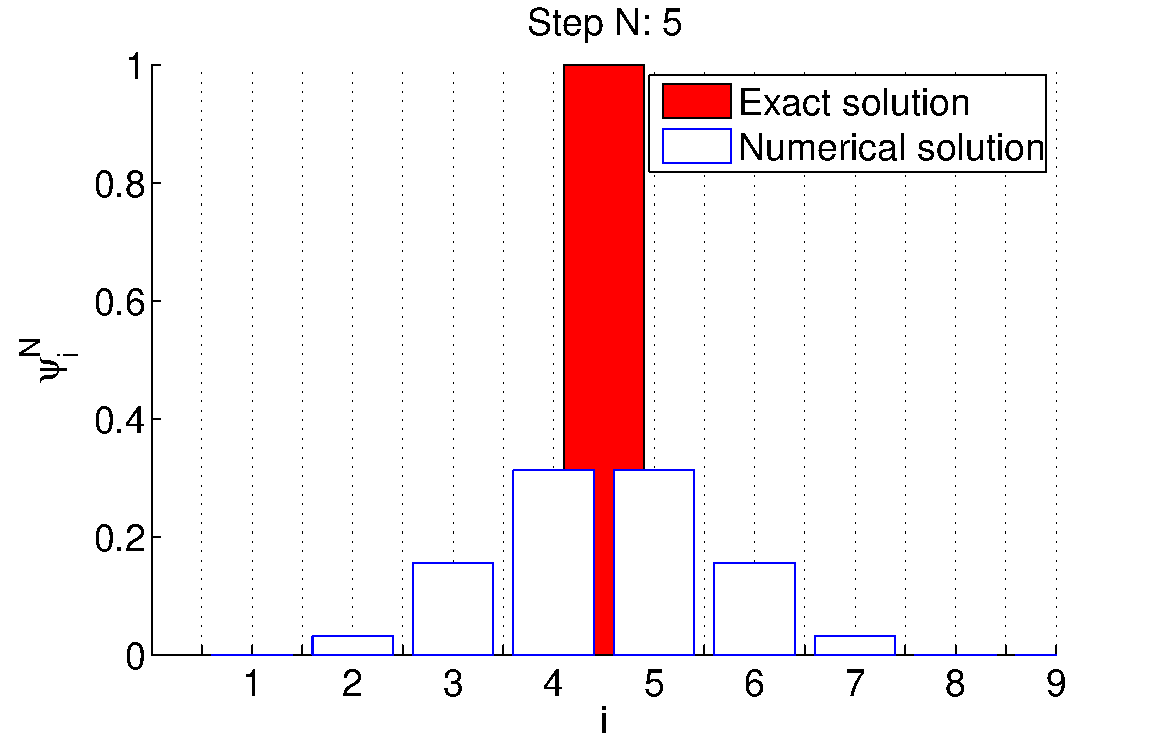
\includegraphics{../presentation/animation/anime5.pdf}}} \\
{\resizebox{\imsize}{!}{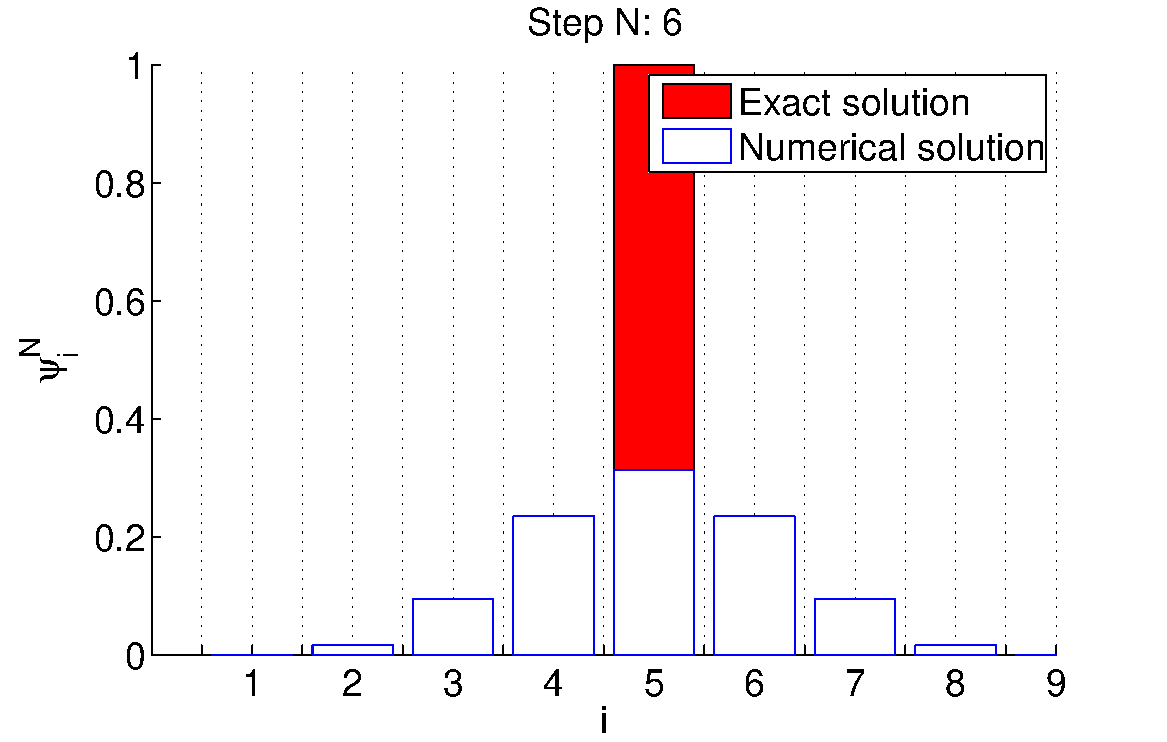
\includegraphics{../presentation/animation/anime6.pdf}}} &
{\resizebox{\imsize}{!}{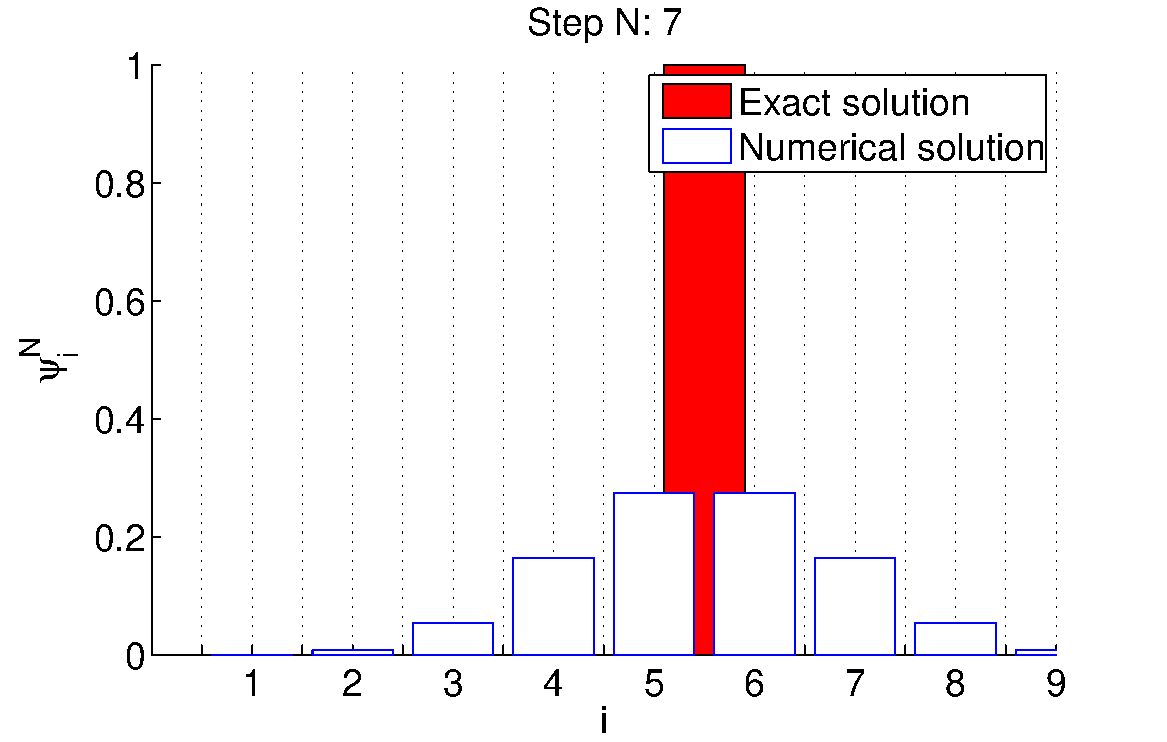
\includegraphics{../presentation/animation/anime7.pdf}}} \\
\end{tabular}
\caption{\label{fig:dif}Example of diffusion when the speed $u=0.5$.}
\end{figure}



\subsection{Anti-diffusion}
To correct for the diffusion in numerical models several techniques were proposed. There is always a trade-off between computing cost and accuracy. In \cite{smolarki}, three anti-diffusive methods are briefly introduced. The first two methods, flux-corrected transport (FCT) \cite{borisbook} and self-adjusting hybrid scheme method (SAHS) \cite{hartenzwas} share high accuracy but also require excessive computing time. Both methods calculate a weighted average of different ordered schemes to deal with diffusion. A third method by Clark and Hall \cite{clarkhall}, the hybrid-type scheme based on a Crowley advection scheme, requires less computing time but is less accurate and might introduce negative values, causing unphysical undershoot. Though these values might be small enough to be neglected, it does violate one of the constraints we set in Section \ref{sec:solvadveq}.

\section{Case study: Smolarkiewicz}
In his 1983 paper, Smolarkiewicz introduces a simple upstream scheme on a staggered grid with iterative corrections for diffusion. At every time step, a simple upstream scheme is used to calculate the advection. This results in the diffusion that we have seen in Figure \ref{fig:diffusion}. Then, the diffusive effect is reversed by a number of iterations using an anti-diffusion velocity $\tilde{u}$.

In step 1 of the algorithm, Smolarkiewicz uses the upstream advection equation on a staggered grid:
\begin{equation}
 \psi_i^{N+1} = \psi_i^N - \Big( F \left( \psi_i^N,\psi_{i+1}^N,u_{i+1/2}^N\right)
-F \left( \psi_{i-1}^N,\psi_{i}^N,u_{i-1/2}^N\right) \Big),\label{eq:noanti}
\end{equation}

where

\begin{equation}
F \left( \psi_i^N,\psi_{i+1}^N,u_{i+1/2}^N\right) =
\Big( \left( u_{i+1/2}^N + \abs{u_{i+1/2}^N} \right) \psi_i^N
+ \left( u_{i+1/2}^N - \abs{u_{i+1/2}^N} \right) \psi_{i+1}^N \Big)
\frac{\Delta t}{2 \Delta x}.
\end{equation}


Here $\psi_i^N$ is the value of $\psi$ at the $i$-th grid point for time step $N$, $\Delta t$ and $\Delta x$ are the time and space increments and the fluxes $F$ are defined at the same staggered points as the velocity values.

For stability we require that

\begin{equation}
\max_{i}\left(\frac{\abs{u_{i+1/2}}\Delta t}{\Delta x}\right) \leq 1
\end{equation}

This also guarantees that the scheme is positive definite: there are no unphysical negative values in a solution at any time.

As we can see in Figure \ref{fig:diffusion}, just applying this upstream scheme will result in a highly smeared out solution after only a few steps. Therefore, in step 2 of the algorithm, this upstream scheme is applied a number of times using an anti-diffusive velocity, which is meant to counter the diffusion of the algorithm. We can therefore write the scheme as

\begin{align}
 \psi_i^{*} &= \psi_i^n - \Big( F \left( \psi_i^n,\psi_{i+1}^n,u_{i+1/2}^n\right)
-F \left( \psi_{i-1}^n,\psi_{i}^n,u_{i-1/2}^n\right) \Big),\label{eq:anti1}\\
 \psi_i^{n+1} &= \psi_i^* - \Big( F \left( \psi_i^*,\psi_{i+1}^*,\tilde{u}_{i+1/2}^n\right)
-F \left( \psi_{*}^n,\psi_{*}^n,\tilde{u}_{i-1/2}^n\right) \Big),\label{eq:anti2}\,
\end{align}

where

\begin{equation}
\tilde{u}_{i+1/2} = \frac{\left(\abs{u_{i+1/2}}\Delta x - \Delta t u_{i+1/2}^2 \right) \left( \psi_{i+1}^*-\psi_i^*\right)}{ \left( \psi_i^*+\psi_{i+1}^*+\epsilon \right) \Delta x}
\end{equation}

We see that \ref{eq:anti1} is the same as \ref{eq:noanti}, only now the result is not directly stored in $\psi^{N+1}$, but in an intermediate vector $\psi^*$. Then we can apply \ref{eq:anti2} any number of times to increase the accuracy of the simulation. In practice, the gain in accuracy decreases with the number of iterations. The exact number of iterations to use depends on the computational resources at hand, Smolarkiewicz suggests using 2 iterations.

\subsection{Implementation}
\label{sec:implementation}
We implement the anti-diffusion scheme in Fortran. For this, we use the method of lines. First, we write out the equations. We see that \ref{eq:anti1} and \ref{eq:anti2} use the same flux operators, only the input velocity vector and system state vector are different. Therefore, we only need to write out \ref{eq:anti1}.

\begin{multline}
\psi_i^* = \psi_i^N - \frac{\Delta t}{2 \Delta x} \bigg( \Big( \left( u_{i+1/2}^N + \abs{u_{i+1/2}^N} \right) \psi_i^N
+ \left( u_{i+1/2}^N - \abs{u_{i+1/2}^N} \right) \psi_{i+1}^N \Big)
\\
- \Big( \left( u_{i-1/2}^N + \abs{u_{i-1/2}^N} \right) \psi_{i-1}^N
+ \left( u_{i-1/2}^N - \abs{u_{i-1/2}^N} \right) \psi_{i}^N \Big) \bigg).
\end{multline}
Collecting terms gives the method of lines representation
\begin{equation}
\begin{split}
\psi_i^* &=
\frac{\Delta t}{2 \Delta x} \left( u_{i-1/2}^N + \abs{u_{i-1/2}^N} \right) \psi_{i-1}^N\\
&+ \left(1 - \frac{\Delta t}{2 \Delta x} \left( u_{i+1/2}^N + \abs{u_{i+1/2}^N} - u_{i-1/2}^N + \abs{u_{i-1/2}^N} \right) \right) \psi_i^N\\
&-\frac{\Delta t}{2 \Delta x} \left( u_{i+1/2}^N - \abs{u_{i+1/2}^N} \right) \psi_{i+1}^N\\
\end{split}
\end{equation}

With substitution of terms

\begin{equation*}
\psi_i^* = \alpha_i \psi_{i-1}^N + \beta_i \psi_i^N +\gamma_i \psi_{i+1}^N, \quad \text{for } i=1,\ldots,M-1,
\end{equation*}
 where we have that
\begin{align*}
\alpha_i &= \frac{\Delta t}{2 \Delta x} \left( u_{i-1/2}^N + \abs{u_{i-1/2}^N} \right),\\
 \beta_i &= \left(1 - \frac{\Delta t}{2 \Delta x} \left( u_{i+1/2}^N + \abs{u_{i+1/2}^N} - u_{i-1/2}^N + \abs{u_{i-1/2}^N} \right) \right),\\
\gamma_i &= -\frac{\Delta t}{2 \Delta x} \left( u_{i+1/2}^N - \abs{u_{i+1/2}^N} \right).
\end{align*}

We can write this in matrix form using Dirichlet boundary conditions as

\begin{equation*}
\begin{bmatrix}\psi_{1}^*\\\psi_{2}^*\\ \vdots \\\psi_{M-2}^*\\\psi_{M-1}^*\end{bmatrix} =
\begin{bmatrix}\beta_1&\gamma_1&&&0\\ \alpha_2&\beta_2&\gamma_2\\ &\ddots&\ddots&\ddots\\&&\alpha_{M-2}&\beta_{M-2}&\gamma_{M-2}\\0&&&\alpha_{M-1}&\beta_{M-1}\\ \end{bmatrix}
\begin{bmatrix}\psi_{1}^N\\\psi_{2}^N\\ \vdots \\\psi_{M-2}^N\\\psi_{M-1}^N\end{bmatrix}
\end{equation*}

or with periodic boundary conditions, so that we only need to store a limited domain for long simulations, as

\begin{equation*}
\begin{bmatrix}\psi_{1}^*\\\psi_{2}^*\\ \vdots \\\psi_{M-2}^*\\\psi_{M-1}^*\end{bmatrix} =\begin{bmatrix}\beta_1&\gamma_1&&&\mathbf{\alpha_1}\\ \alpha_2&\beta_2&\gamma_2\\ &\ddots&\ddots&\ddots\\&&\alpha_{M-2}&\beta_{M-2}&\gamma_{M-2}\\ \mathbf{\gamma_{M-1}}&&&\alpha_{M-1}&\beta_{M-1}\\ \end{bmatrix}
\begin{bmatrix}\psi_{1}^N\\\psi_{2}^N\\ \vdots \\\psi_{M-2}^N\\\psi_{M-1}^N\end{bmatrix}
\end{equation*}

The values of $\psi^*$ can be obtained very efficiently from those of $\psi^N$ using a sparse matrix vector multiplication. It follows that we can apply this matrix-vector multiplication also to \ref{eq:anti2}, where we substitute $u \rightarrow \tilde{u}$, $\psi^N \rightarrow \psi^*$, $\psi^* \rightarrow \psi^{N+1}$ in case we only run one iteration of \ref{eq:anti2}. If we run more than one iteration, we should update the intermediate vector $\psi^*$ and the anti-diffusion velocity $\tilde{u}$ at each iteration.

Note that the tri-diagonal matrix is only useful for the one dimensional case. If we apply Smolarkiewicz' anti-diffusion scheme in two dimensions, we need to take into account two extra neighboring grid points for every grid point $\psi_{ij}$. Thus, we get the collection of terms

\begin{align*}
\psi_{ij}^* &=
\frac{\Delta t}{2 \Delta y} \left( v_{i,j-1/2}^N + \abs{v_{i,j-1/2}^N} \right) \psi_{i,j-1}^N\\
&+\frac{\Delta t}{2 \Delta x} \left( u_{i-1/2,j}^N + \abs{u_{i-1/2,j}^N} \right) \psi_{i-1,j}^N\\
&+ \Big(1 - u_{i+1/2,j}^N - \abs{u_{i+1/2,j}^N} + u_{i-1/2,j}^N - \abs{u_{i-1/2,j}^N} - v_{i,j+1/2}^N - \abs{v_{i,j+1/2}^N} \\
&+ v_{i,j-1/2}^N - \abs{v_{i,j-1/2}^N} \Big) \psi_i^N\\
&-\frac{\Delta t}{2 \Delta x} \left( u_{i+1/2,j}^N - \abs{u_{i+1/2,j}^N} \right) \psi_{i+1,j}^N\\
&-\frac{\Delta t}{2 \Delta y} \left( v_{i,j+1/2}^N - \abs{v_{i,j+1/2}^N} \right) \psi_{i,j+1}^N,\\
\end{align*}

substitution gives

\begin{align*}
\alpha_i &= \frac{\Delta t}{2 \Delta y} \left( v_{i,j-1/2}^N + \abs{v_{i,j-1/2}^N} \right),\\
\beta_i &= \frac{\Delta t}{2 \Delta x} \left( u_{i-1/2,j}^N + \abs{u_{i-1/2,j}^N} \right),\\
\gamma_i &= \Big(1 - u_{i+1/2,j}^N - \abs{u_{i+1/2,j}^N} + u_{i-1/2,j}^N - \abs{u_{i-1/2,j}^N} - v_{i,j+1/2}^N - \abs{v_{i,j+1/2}^N} \\
&+ v_{i,j-1/2}^N - \abs{v_{i,j-1/2}^N} \Big),\\
\delta_i &= -\frac{\Delta t}{2 \Delta x} \left( u_{i+1/2,j}^N - \abs{u_{i+1/2,j}^N} \right),\\
\epsilon_i &= -\frac{\Delta t}{2 \Delta y} \left( v_{i,j+1/2}^N - \abs{v_{i,j+1/2}^N} \right).
\end{align*}

\begin{equation*}
\psi_{ij}^* = \alpha_{ij} \psi_{i,j-1}^N + \beta_{ij} \psi_{i-1,j}^N +\gamma_{ij} \psi_{i,j}^N +\delta_{ij} \psi_{i+1,j}^N + \epsilon_{ij} \psi_{i,j+1}^N, \quad \text{for } i,j=1,\ldots,M-1,
\end{equation*}

which gives a pentadiagonal sparse matrix. Again, we can use sparse matrix vector multiplication. In the three-dimensional case, we would get a septadiagonal matrix.

In general, we find a numerical solution using the following algorithm

\IncMargin{1em}
\begin{algorithm}[H]
\SetKwData{Iter}{iter}\SetKwData{Mone}{mat1}\SetKwData{Mtwo}{mat2}
\SetKwData{Steps}{tsteps}
\SetKwFunction{MMat}{ComputeMatrix}\SetKwFunction{MMult}{MatrixMultiplication}
\SetKwFunction{CADV}{ComputeAntidiffusionVelocity}
\SetKwInOut{Input}{input}\SetKwInOut{Output}{output}
\Input{Initial state $\psi^0$, velocities $u$, \Iter, \Steps, $\Delta x$, $\Delta t$}
\Output{Final state $\psi^N$}
\BlankLine
$\psi \leftarrow \psi^0$\;
\Mone $\leftarrow$ \MMat{$u,\Delta x, \Delta t$}\;
\For{$i \leftarrow 1$ \KwTo \Steps}{
$\psi \leftarrow$ \MMult{\Mone,$\psi$}\;
\For{$j \leftarrow 1$ \KwTo \Iter}{
$\widetilde{u} \leftarrow$ \CADV{$\psi,u$}\;
\Mtwo $\leftarrow$ \MMat{$\widetilde{u},\Delta x, \Delta t$}\;
$\psi \leftarrow$ \MMult{\Mtwo,$\psi$}\;
}
}
$\psi^N \leftarrow \psi$\;
\end{algorithm}
\DecMargin{1em}





\subsection{Numerical results}
We have applied the anti-diffusive scheme to the one dimensional case and the two dimensional case. We will first discuss some results for the one dimensional case.


\subsubsection{Results in one dimension}
We have developed a graphical user interface (GUI) in Matlab (Figure \ref{fig:1dgui}) so that we can test different configurations on the fly. In the GUI, we can check for instabilities and set the initial condition and the velocity vector very easily. Using this GUI we find that the scheme is indeed both volume preserving and positive definite.

We can visualize the effect of using anti-diffusion iterations by again taking the problem in Figure \ref{fig:dif}, but now applying two anti-diffusion iterations at each time step. In the blue bars, we have the original diffused numerical solution. In the black bars we have the anti-diffusive solution. We see that the anti-diffusive solution is more concentrated around the exact solution.

Is is interesting to visualize the anti-diffusion vector to see what exactly is going on. In Figure \ref{fig:antivec} we see the anti-diffusion vector for a system where there the exact solution lies around $\psi_{25}$. The substance is moving to the right at a constant speed $u=0.5$, which makes this simulation similar to those in Figures \ref{fig:dif} and \ref{fig:antidif}. We see that whereas the velocity vector is positive everywhere, the anti-diffusive velocity vector is negative in front of the exact solution, thus pushing the substance back, and positive behind the exact solution, thus pushing the substance forward. In fact, the substance is compressed around the exact solution, which helps preserve the shape of the substance.



\begin{figure}[htp]
\renewcommand{\imsize}{0.3\textwidth}
\begin{tabular}{ccc}
{\resizebox{\imsize}{!}{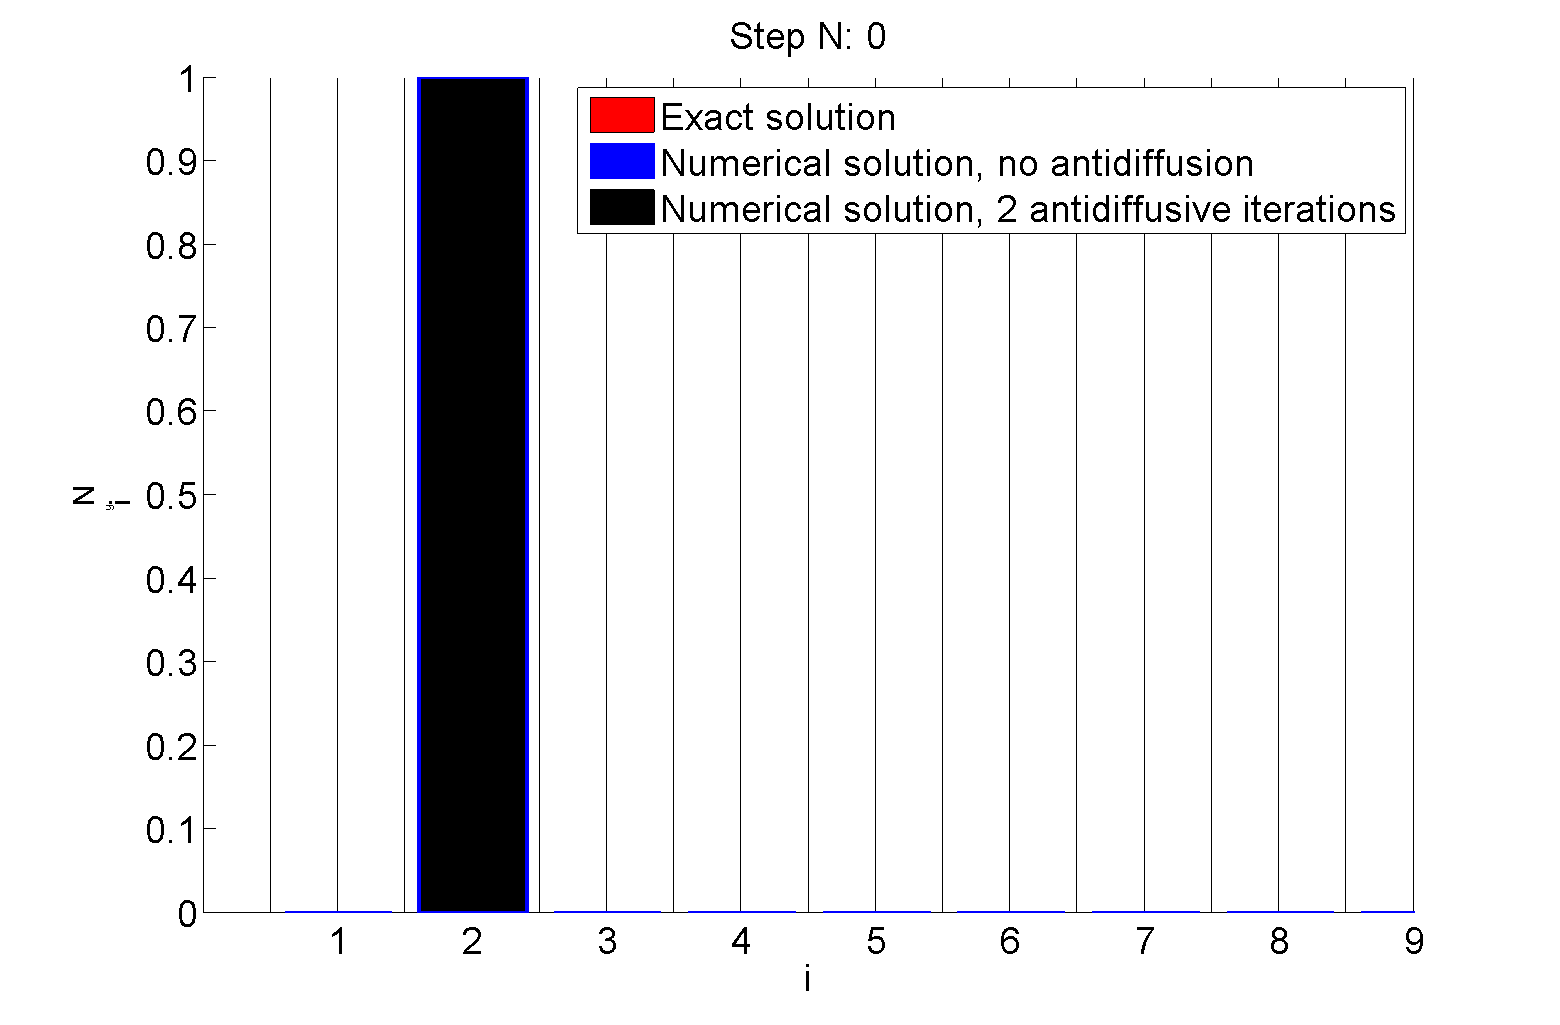
\includegraphics{../presentation/animation/aanime0-eps-converted-to.pdf}}} &
{\resizebox{\imsize}{!}{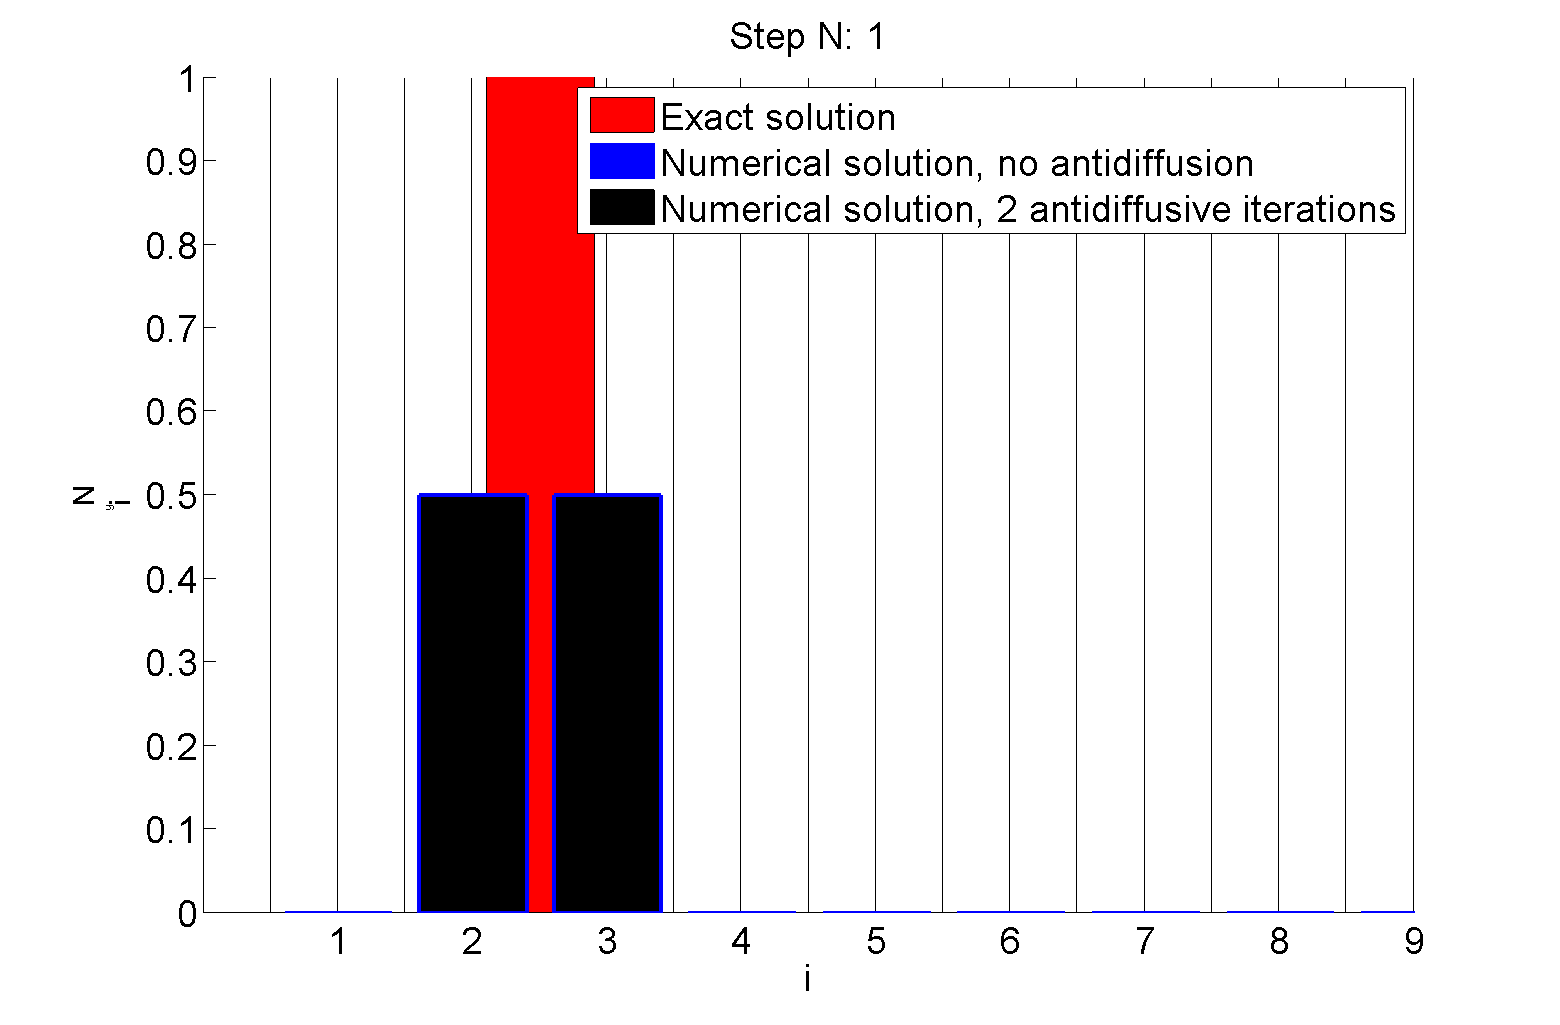
\includegraphics{../presentation/animation/aanime1-eps-converted-to.pdf}}} &
{\resizebox{\imsize}{!}{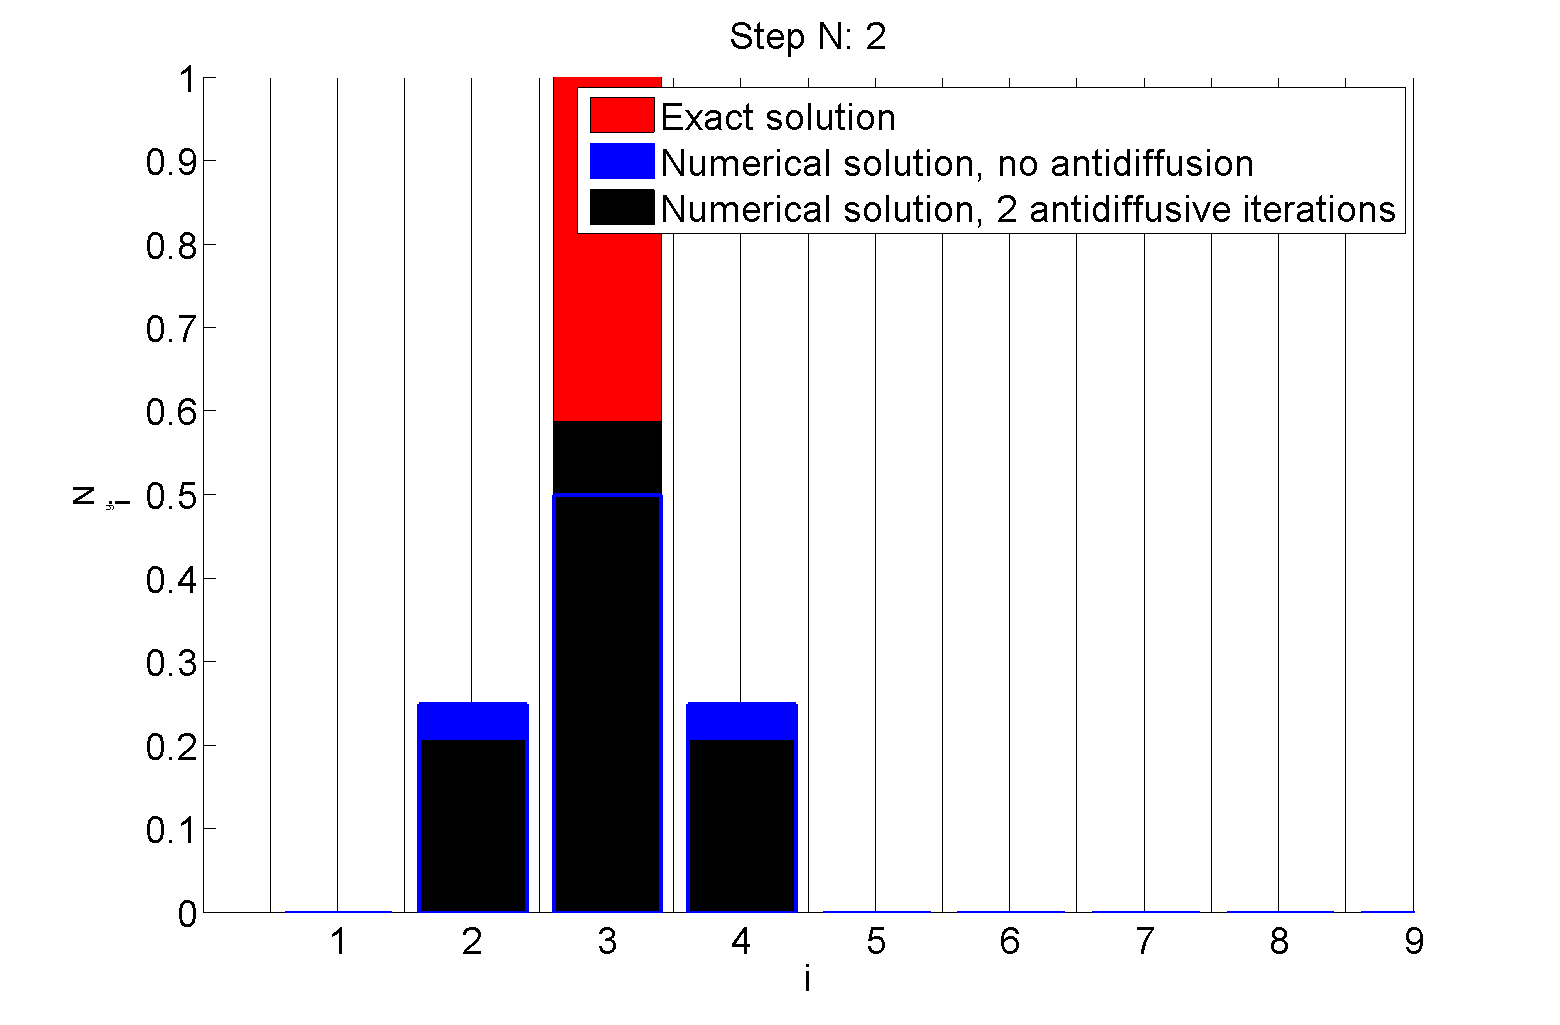
\includegraphics{../presentation/animation/aanime2-eps-converted-to.pdf}}} \\
{\resizebox{\imsize}{!}{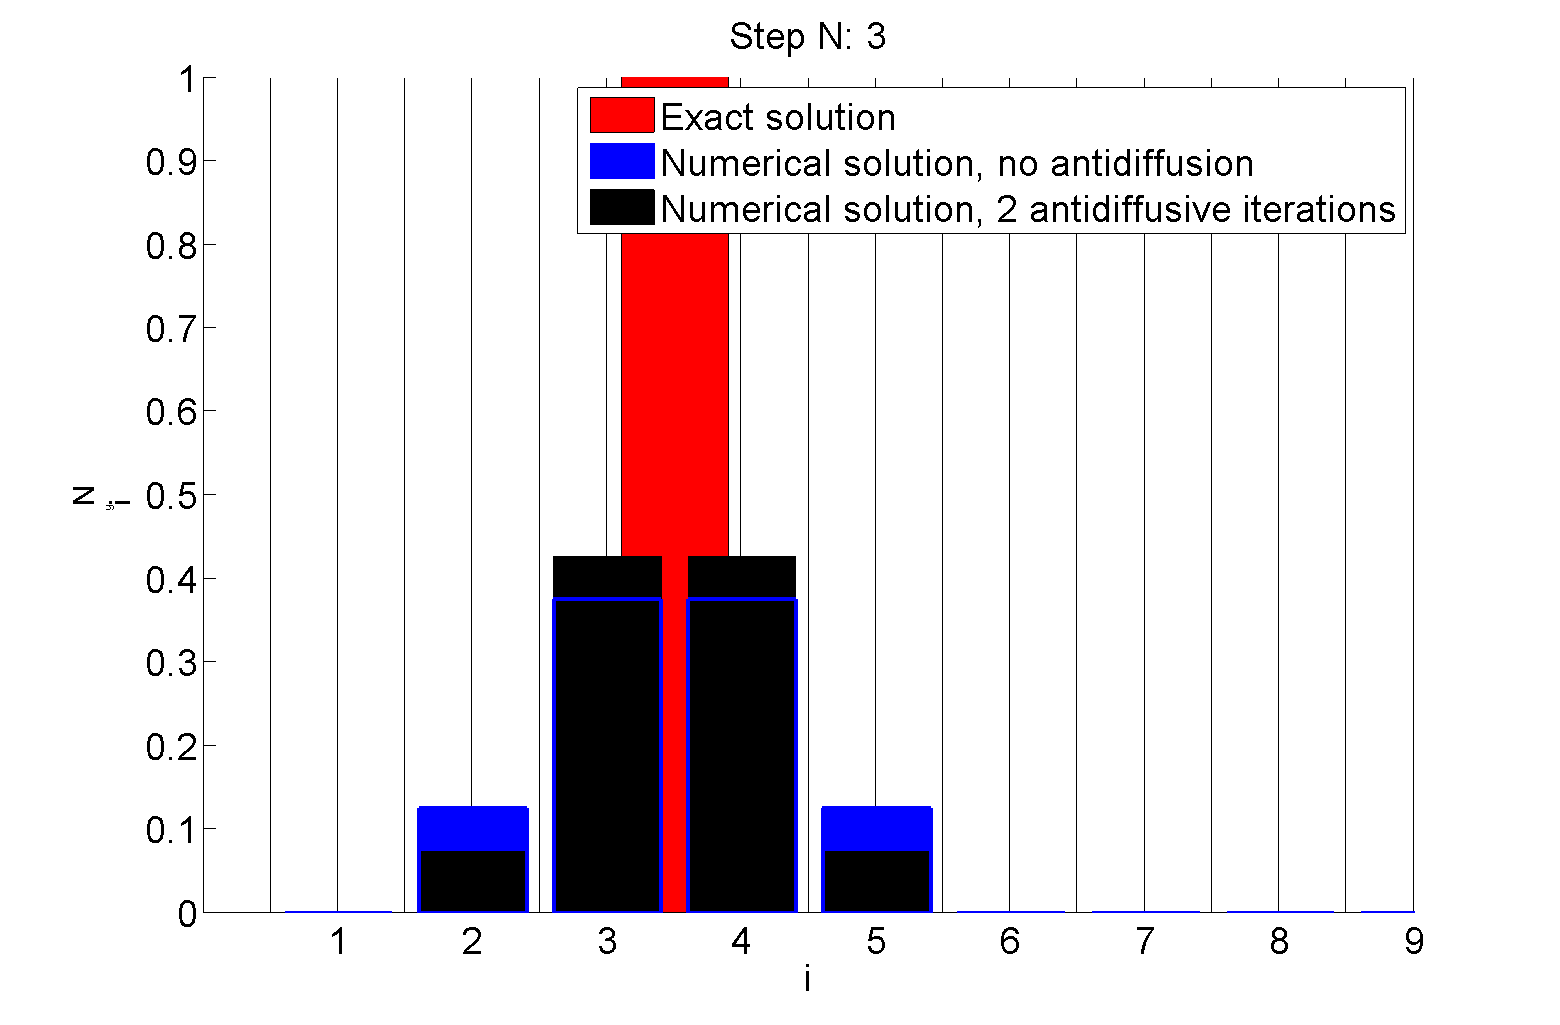
\includegraphics{../presentation/animation/aanime3-eps-converted-to.pdf}}} &
{\resizebox{\imsize}{!}{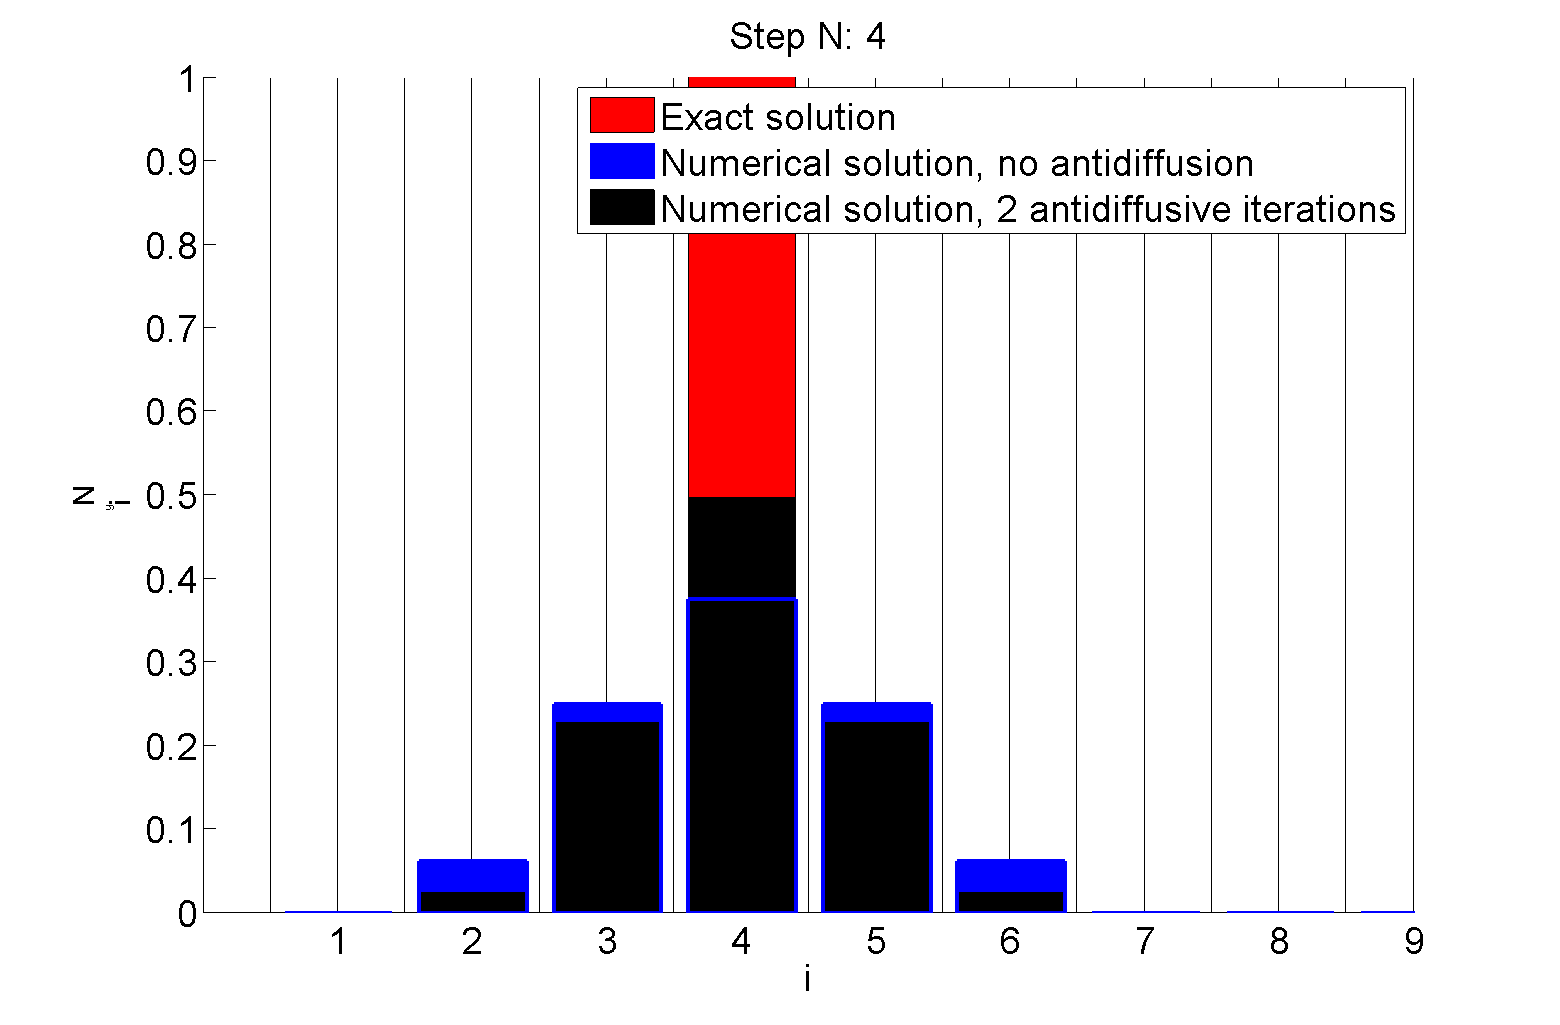
\includegraphics{../presentation/animation/aanime4-eps-converted-to.pdf}}} &
{\resizebox{\imsize}{!}{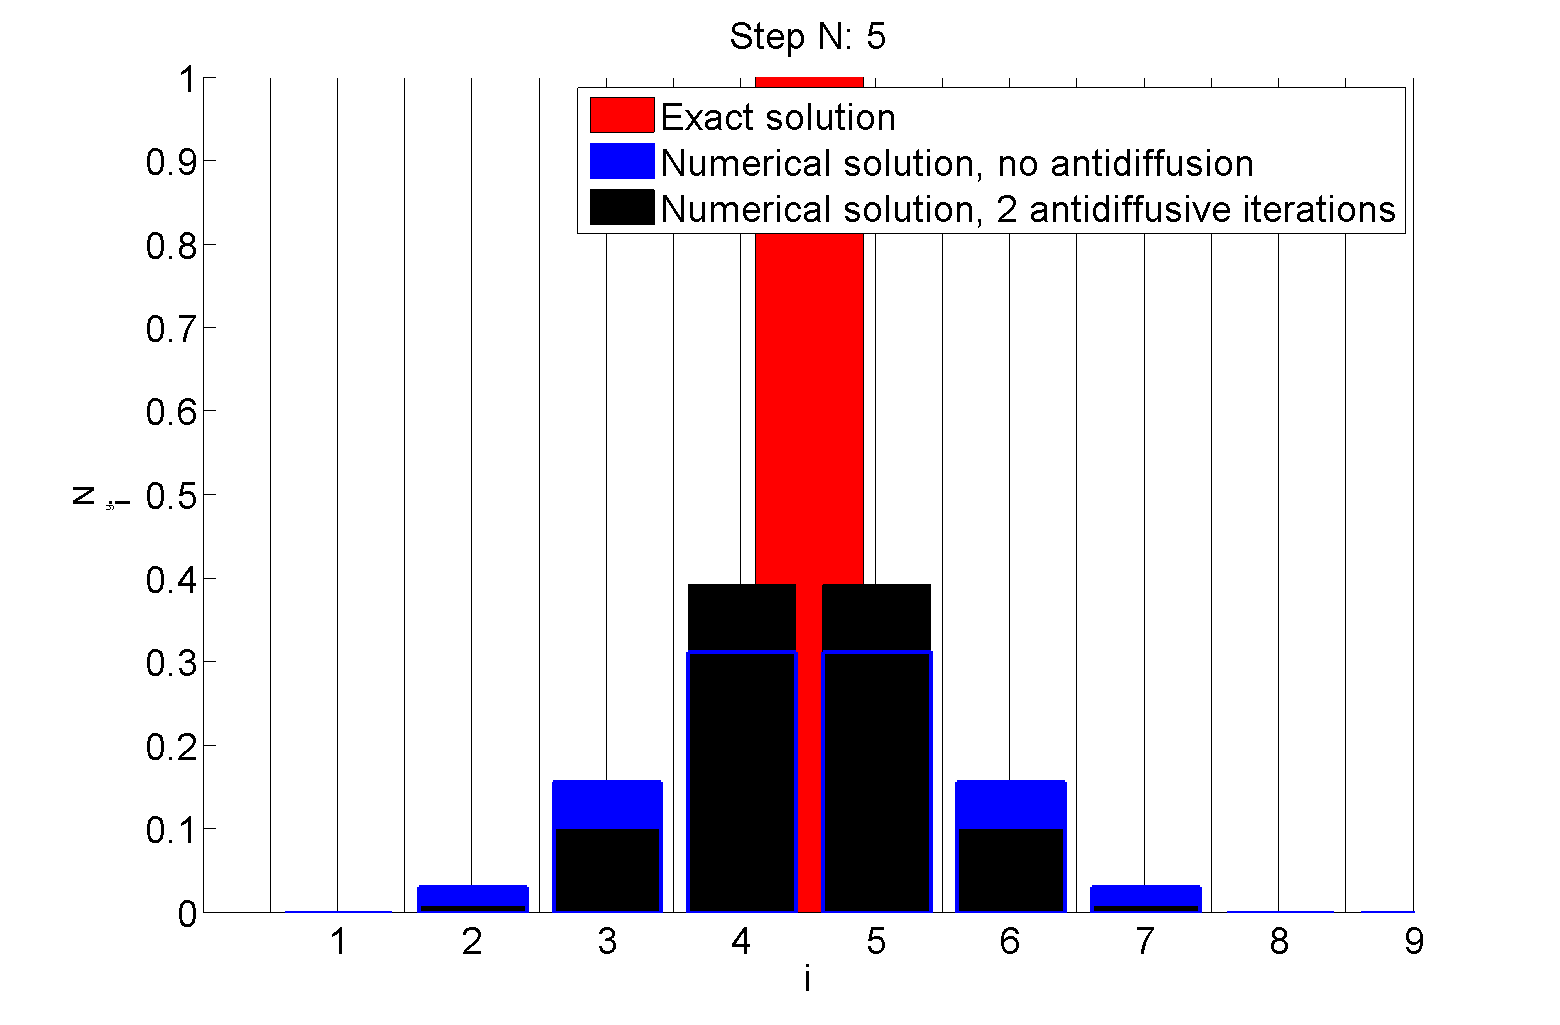
\includegraphics{../presentation/animation/aanime5-eps-converted-to.pdf}}} \\
{\resizebox{\imsize}{!}{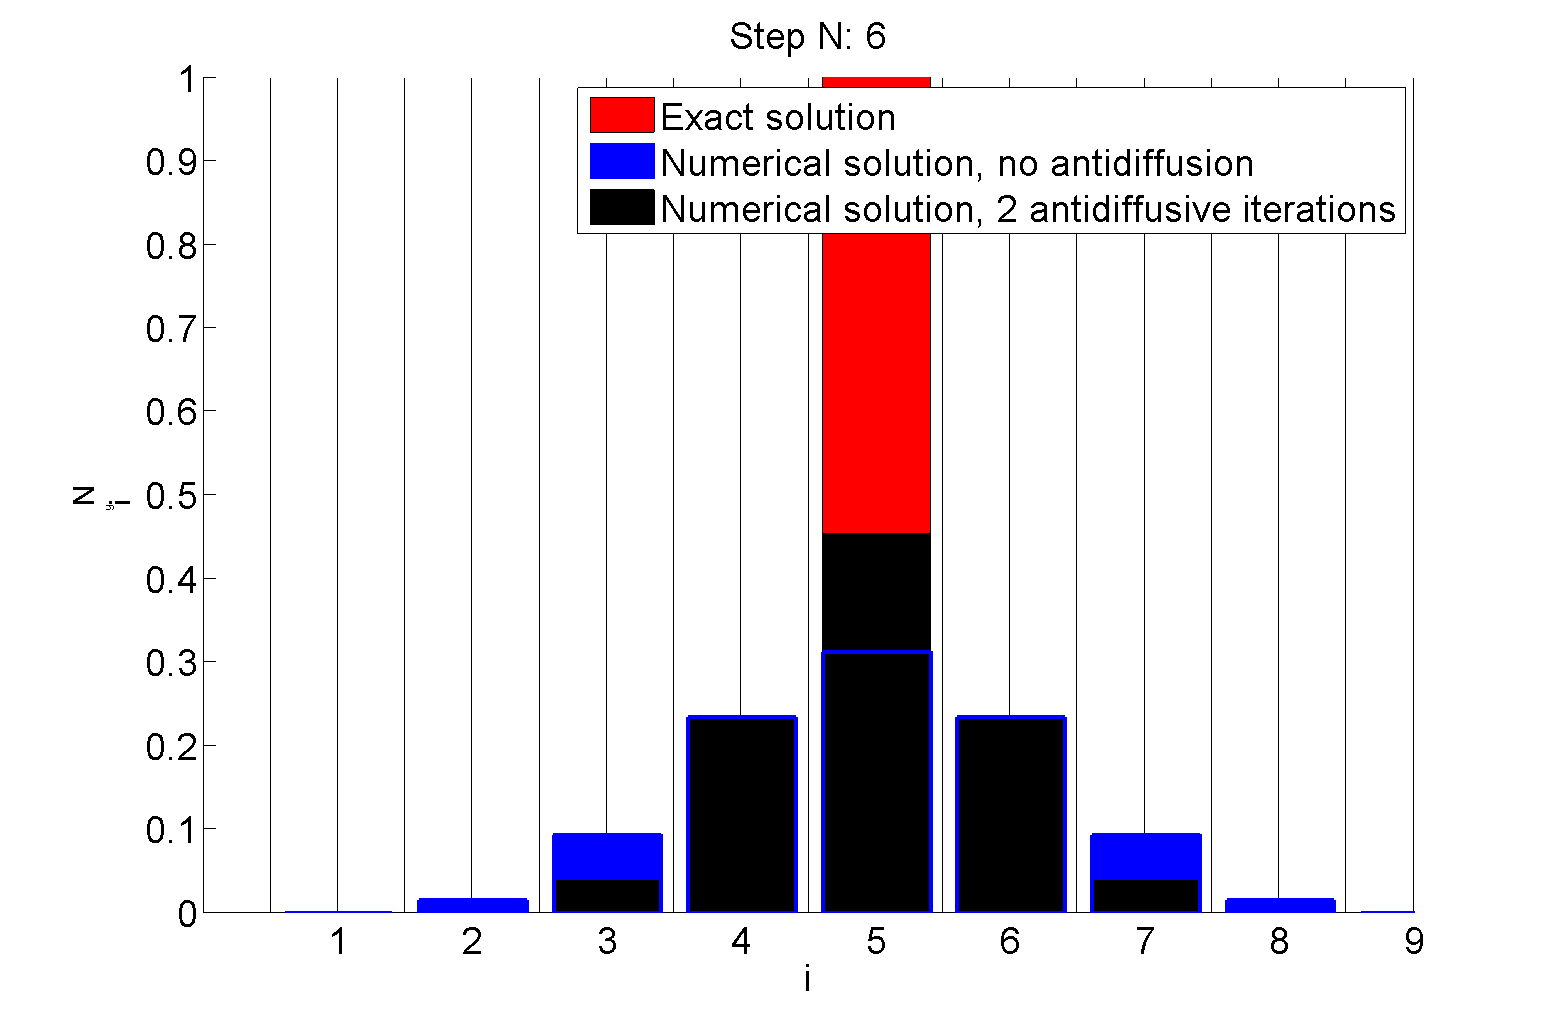
\includegraphics{../presentation/animation/aanime6-eps-converted-to.pdf}}} &
{\resizebox{\imsize}{!}{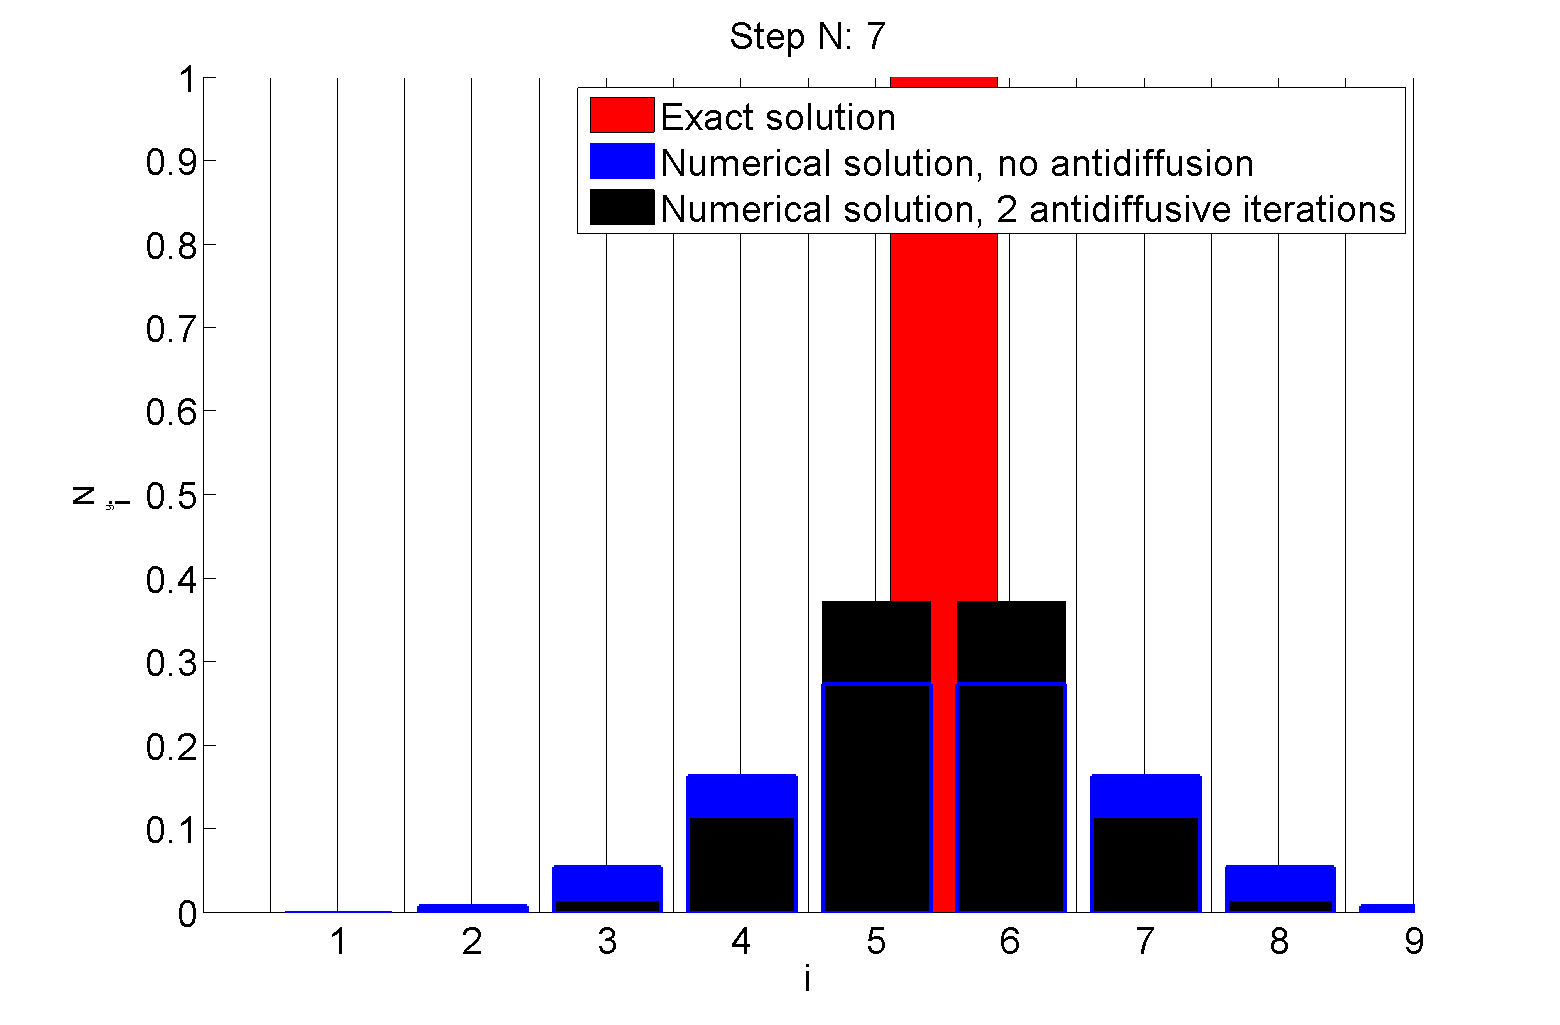
\includegraphics{../presentation/animation/aanime7-eps-converted-to.pdf}}} \\
\end{tabular}
\caption{\label{fig:antidif}Example of antidiffusion when the speed $u=0.5$.}
\label{fig:diffusion}
\end{figure}

\begin{figure}
\centering
 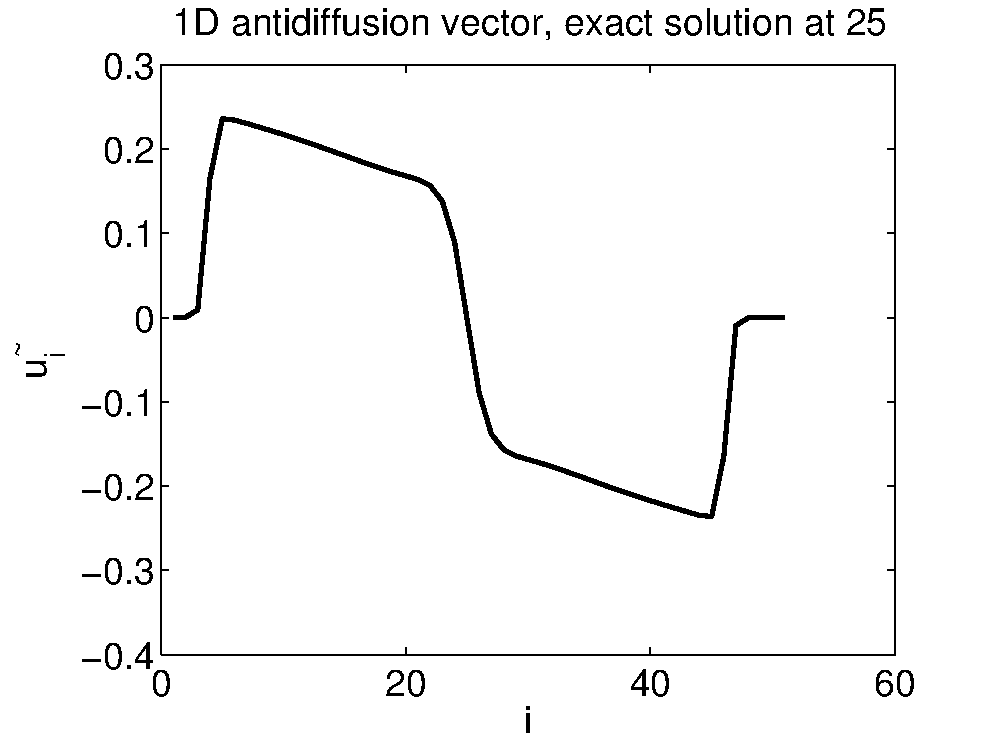
\includegraphics[width=0.6\textwidth]{../presentation/ad1d.pdf}
\caption{Anti-diffusion vector in one dimension}
\label{fig:antivec}
\end{figure}


We find that when we use anti-diffusive iterations, the diffusion is much smaller than in the case where we just apply the basic upstream scheme. We see this very clearly in Figure~\ref{fig:maxs}, where we have plotted the maximum value of the simulation as a function of the time step $N$. When we do not use anti-diffusion, the maximum value rapidly drops to 0, when we use 3 anti-diffusion iterations, the maximum value drops to 0.5, but then remains constant around that value. In this example, the move from 2 to 3 anti-diffusion iterations adds relatively little to the validity of the simulation, compared to the extra computational cost.

In Figure~\ref{fig:local} we see that without anti-diffusion iterations, the smearing causes interactions between pockets which are not meant to interact. We start with three independent substance pockets. After 100 time steps, diffusion has caused the three peaks to merge (blue line), whereas anti-diffusion (black line) preserves the local character of the pockets.



\begin{figure}[htp]
\centering
 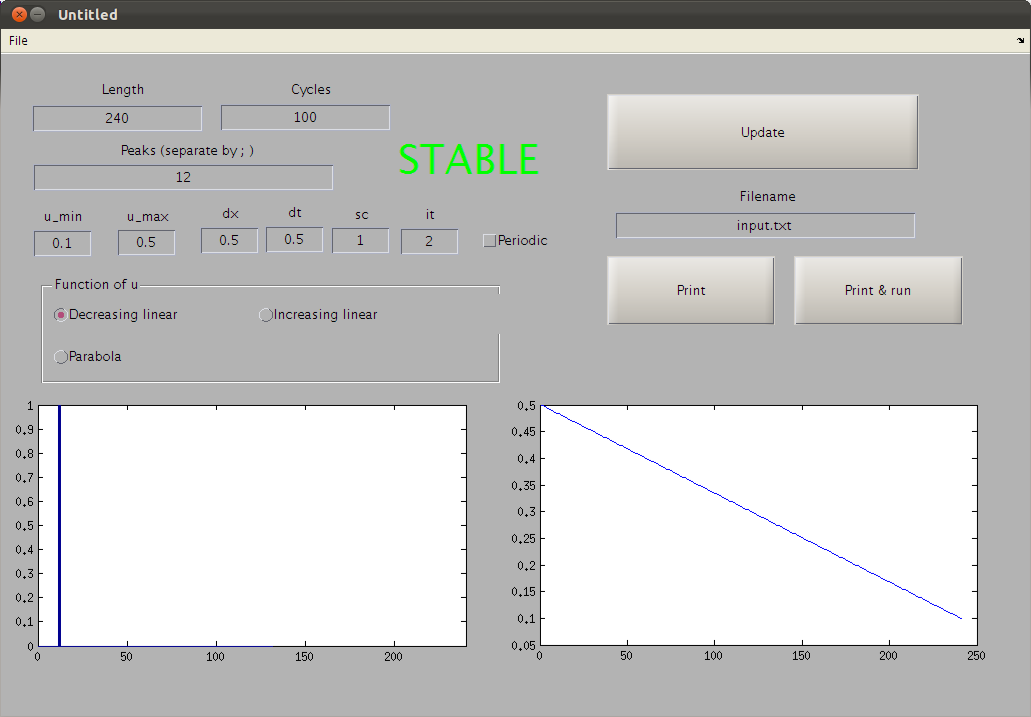
\includegraphics[width=0.8\textwidth]{1dscreenshot.png}
 \caption{Matlab GUI for one dimensional case. We can set the velocity vector $u$, the initial condition $\psi^0$ and a range of other parameters.}
 \label{fig:1dgui}
\end{figure}

\begin{figure}[htp]
\centering
 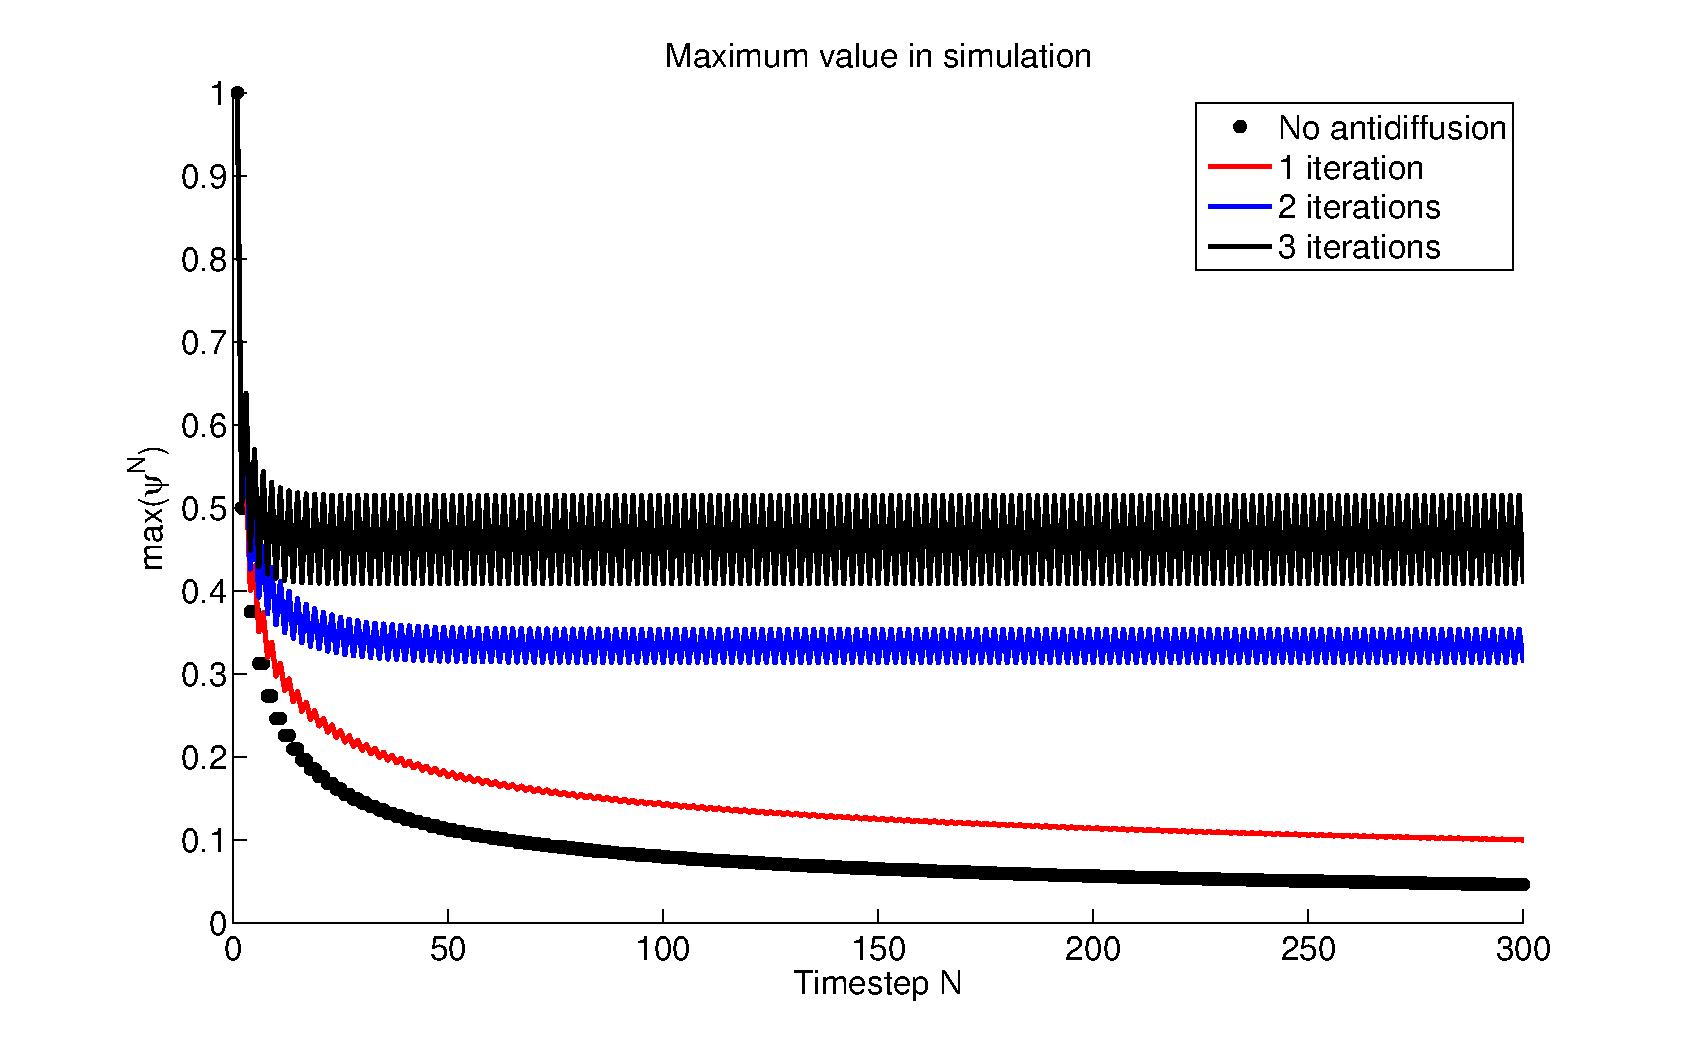
\includegraphics[width=0.8\textwidth]{maxs}
 \caption{Maximum value in the simulation when running with 0, 1, 2 or 3 anti-diffusive iterations.}
 \label{fig:maxs}
\end{figure}


\begin{figure}[htp]
\centering
 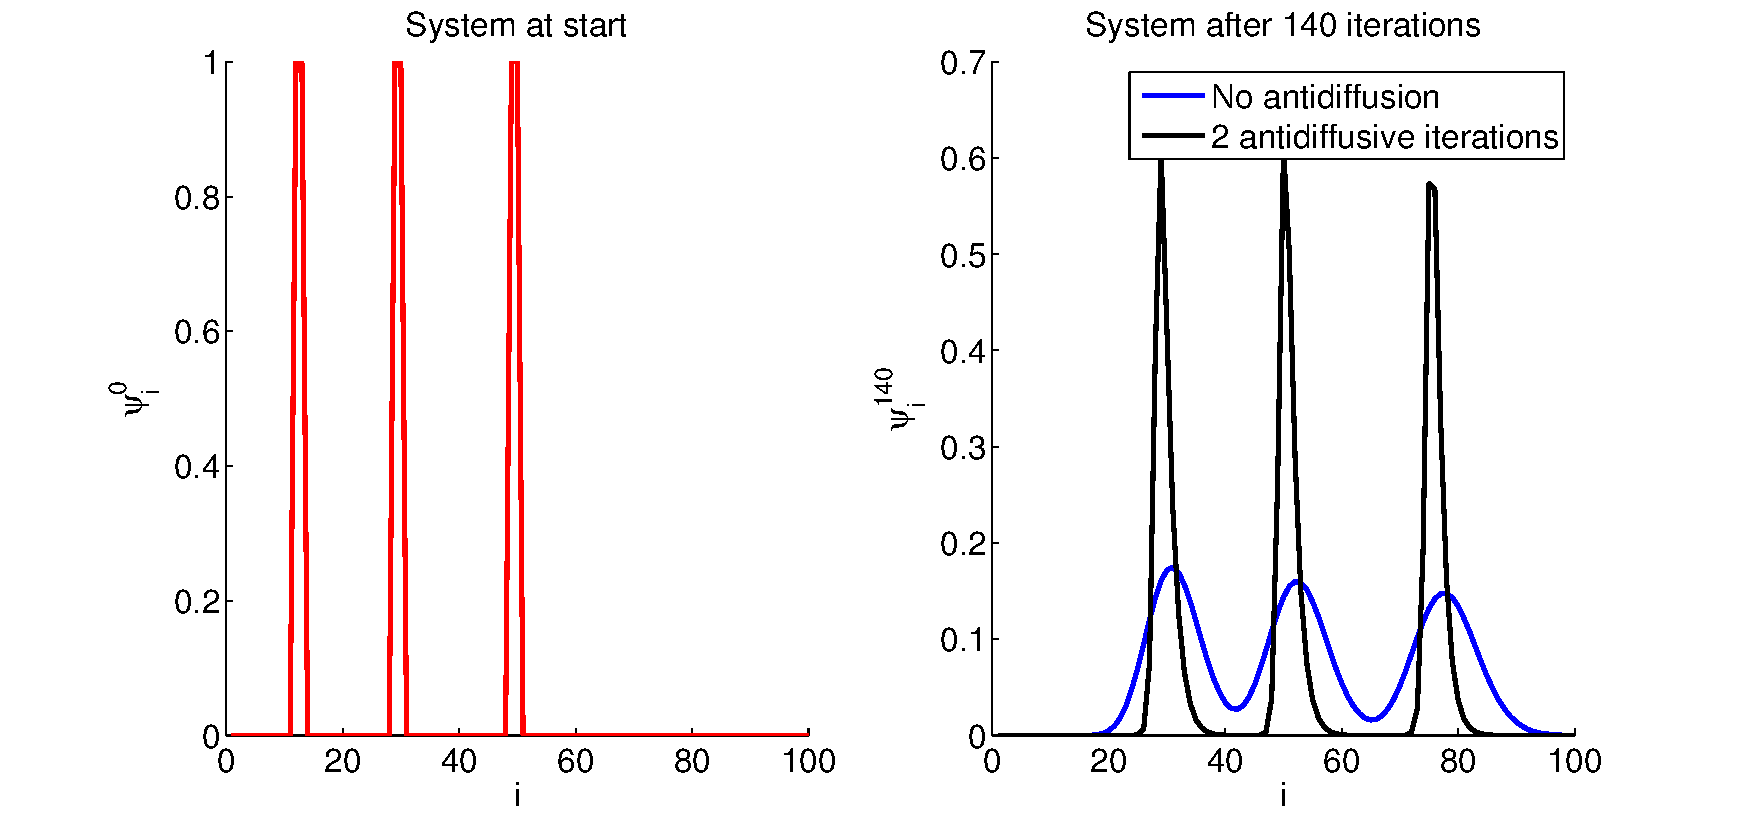
\includegraphics[width=0.8\textwidth]{../presentation/animation/peaks-eps-converted-to.pdf}
 \caption{Interactions between neighboring pockets.}
\label{fig:local}
\end{figure}

\subsubsection{Results in two dimensions}

As we have seen in Section \ref{sec:implementation}, we can implement Smolarkiewicz' scheme in two dimensions as well as in one dimension. As for the one dimensional simulations, we have built a Matlab GUI (Figure \ref{fig:2dgui}). We will show the results of a rotating cone simulation in two dimensions. The cone starts at $(25\Delta x, 75\Delta y)$ and rotates around the center $(50 \Delta x, 50 \Delta y)$ in a $100 \Delta x \times 100 \Delta y$ grid. The initial cone has a maximum value of 3.87. The scheme is stable with $\Delta x = \Delta y = 1$ and $\Delta t = 0.1$. With an angular velocity of $\omega = 0.1$, the velocity components are $u=-\omega(y-y_0)$ and $v=\omega(x-x_0)$, where $(x_0,y_0)$ is the center $(50 \Delta x, 50 \Delta y)$. These parameters are the same as in \cite{smolarki}. One full rotation around the center is equivalent to 628 time steps.

Again, it is interesting to take a look at the anti-diffusion vectors (Figure \ref{fig:antivec2d}). On the left, we have the initial condition, the cone around $(25\Delta x, 75\Delta y)$. In the middle we have the vertical anti-diffusion velocity vector, to the right we have the horizontal anti-diffusion velocity vector. From the anti-diffusion vectors we see that this cone will move counterclockwise. Note that these figures are very similar to Figure \ref{fig:antivec}.

If we take a look at the simulation after one full rotation (Figure \ref{fig:rotcone}, we see that there is almost nothing left of the cone when we don't use anti-diffusive iterations. If we do however use two anti-diffusive iterations, the cone preserves its shape quite well, thus showing results similar to those in Figure \ref{fig:maxs}.

\begin{figure}
\centering
 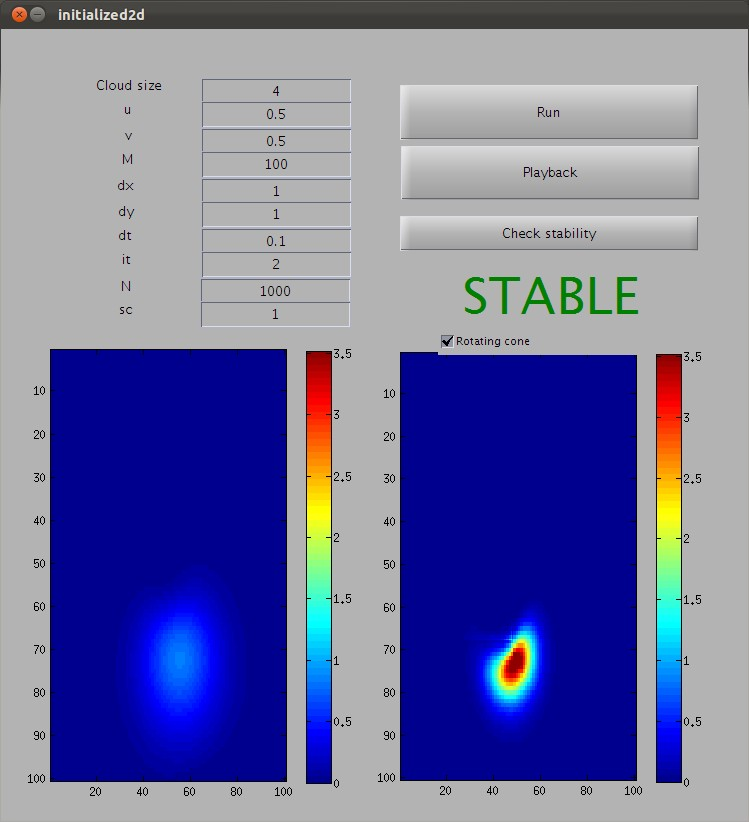
\includegraphics[width=0.8\textwidth]{2dscreenshot.jpg}
 \caption{Matlab GUI for two dimensional case. We can set the velocity vectors $u$ and $v$, the initial condition $\psi^0$ and a range of other parameters. We can view the results of the simulation directly.}
 \label{fig:2dgui}
\end{figure}

\begin{figure}
\centering
 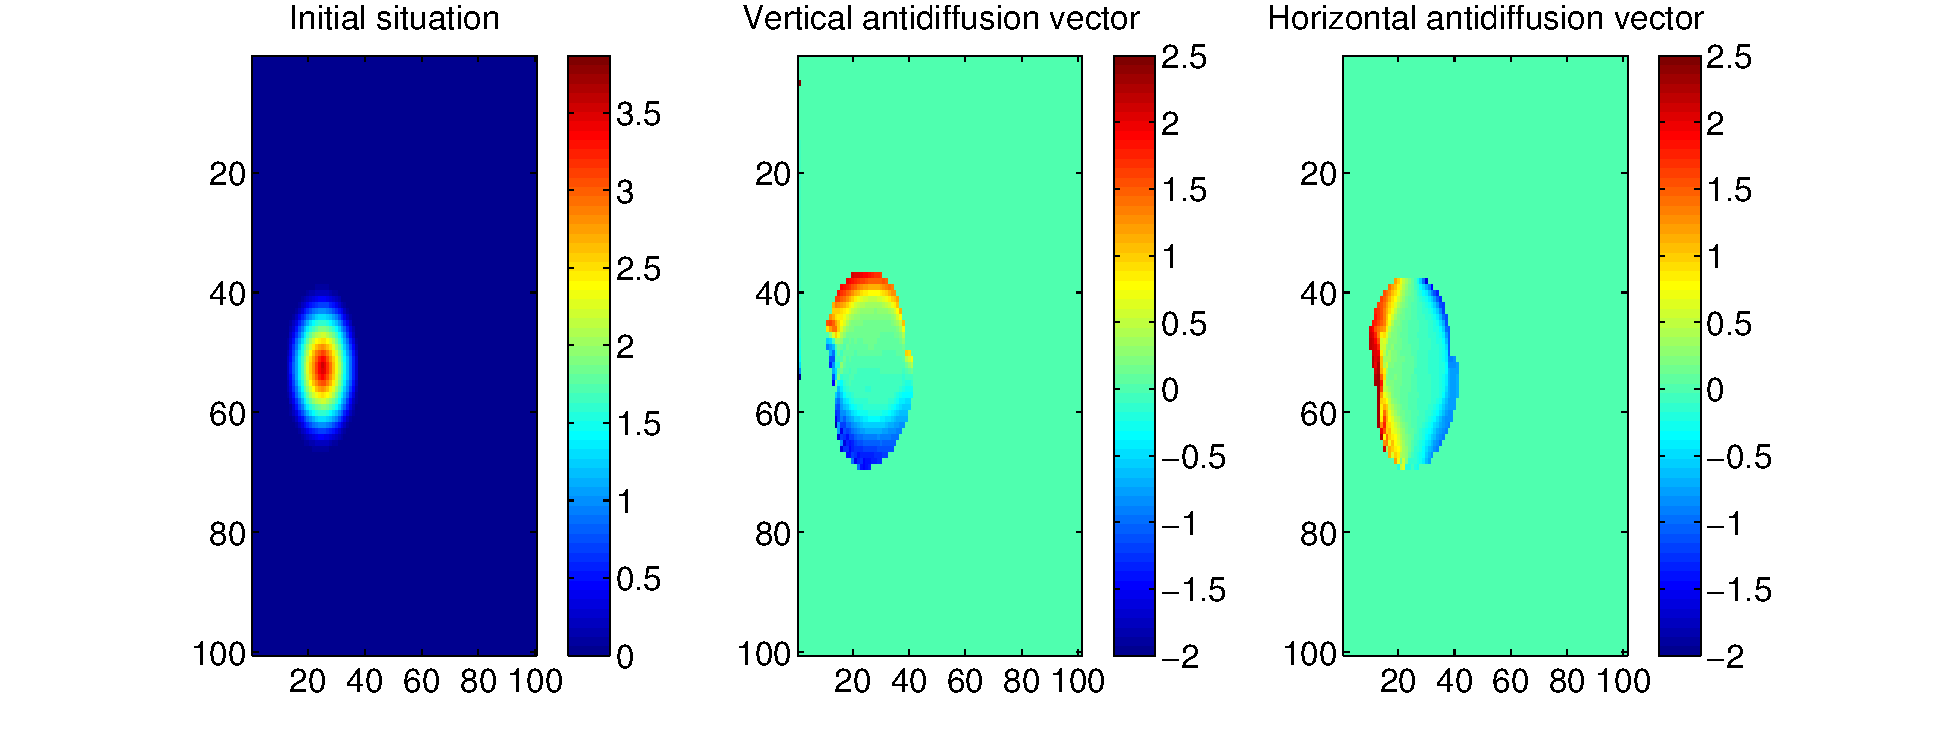
\includegraphics[width=\textwidth]{../presentation/ad2d.pdf}
\caption{Anti-diffusion vector in two dimensions}
\label{fig:antivec2d}
\end{figure}


\begin{figure}
\centering
 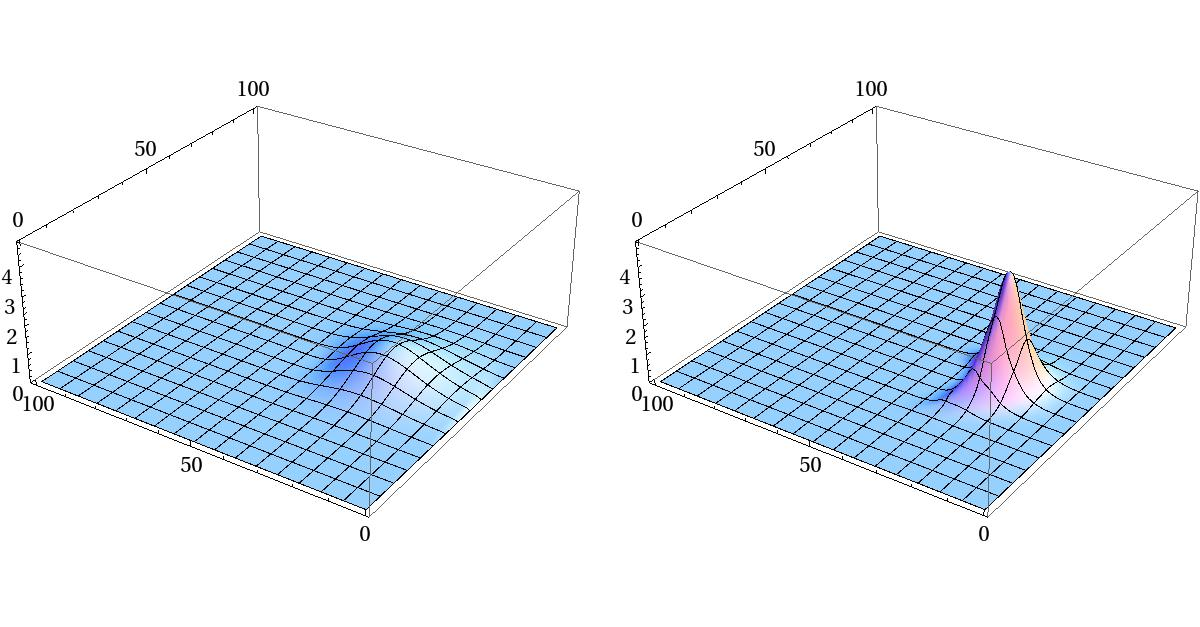
\includegraphics[width=\textwidth]{../presentation/animation2/anim-64}
\caption{Rotating cone simulation after one full rotation. No anti-diffusion (left) and two anti-diffusive iterations (right).}
\label{fig:rotcone}
\end{figure}


\section{Current state of research}
Since Smolarkiewicz' paper in 1983, there are numerous improvements and alternatives developed to solve the advection equation for larger and more complex grids. Examples of this are the methods on a reduced grid developed by Spee et al. in 1997 \cite{spee}. The reduced grid is a grid with the shape of the globe, except that there are less cells near the poles to avoid the well known pole-singularity. Figure~\ref{fig:redgrid} gives an illustration of this reduced grid.

\begin{figure}[htp]
\centering
\renewcommand{\imsize}{0.75\textwidth}%
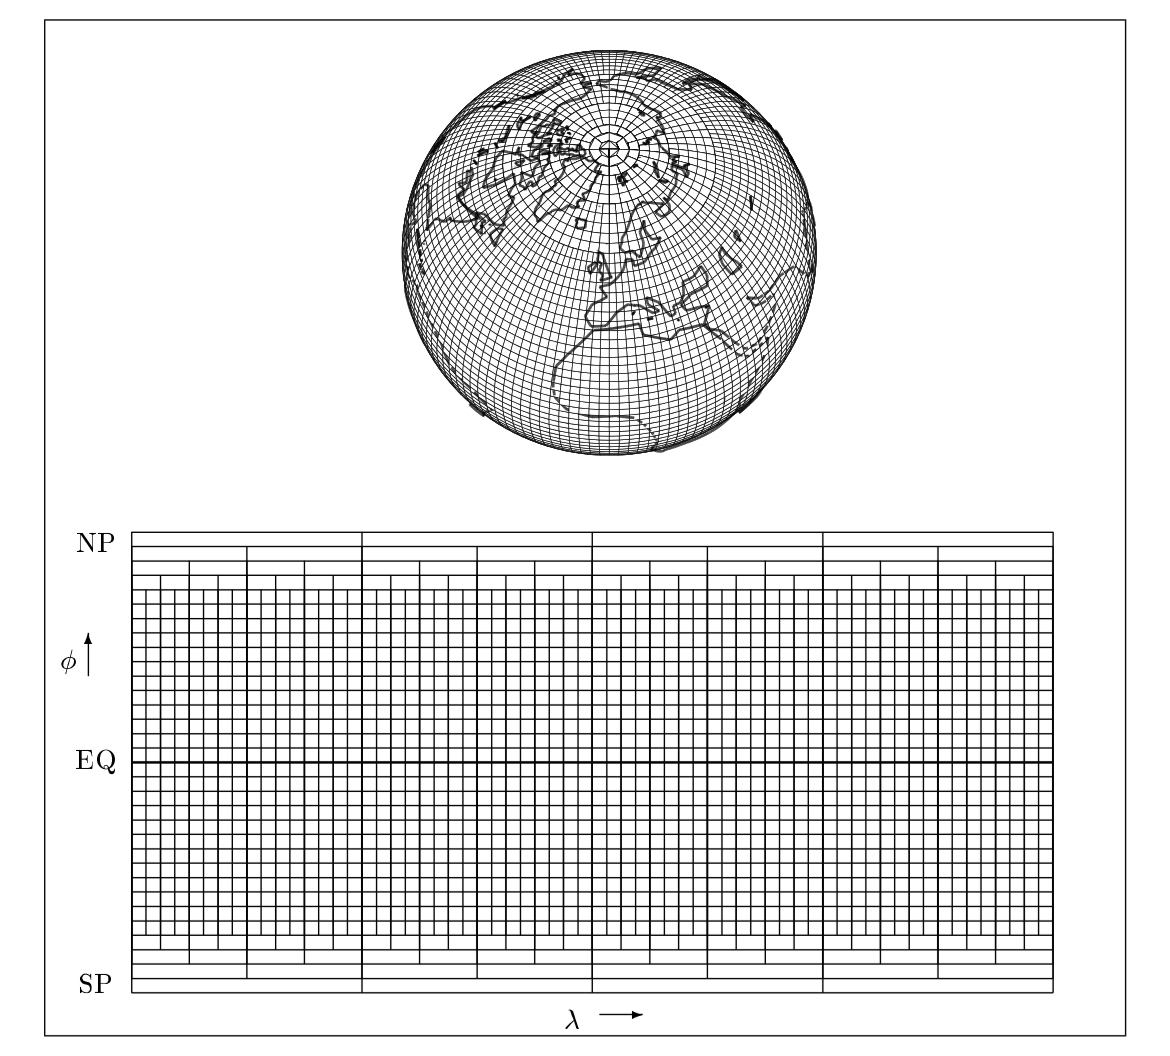
\includegraphics[width=\imsize]{figures/globe}%
\caption{\label{fig:redgrid} Illustration of the reduced grid as used by Spee et al. \cite{spee}.}
\end{figure}

Another example is the spherical geodesic grids used by Lipscomb and Ringler in 2005 \cite{lipscomb}. Figure~\ref{fig:hexpent} shows for example the spherical hexagonal-pentagonal grid, this grid consists of 20 spherical triangles, which in turn can be split in 5 groups of 4 triangles and as the figure shows these groups form rectangles.

\begin{figure}[htp]
\centering
\renewcommand{\imsize}{0.75\textwidth}
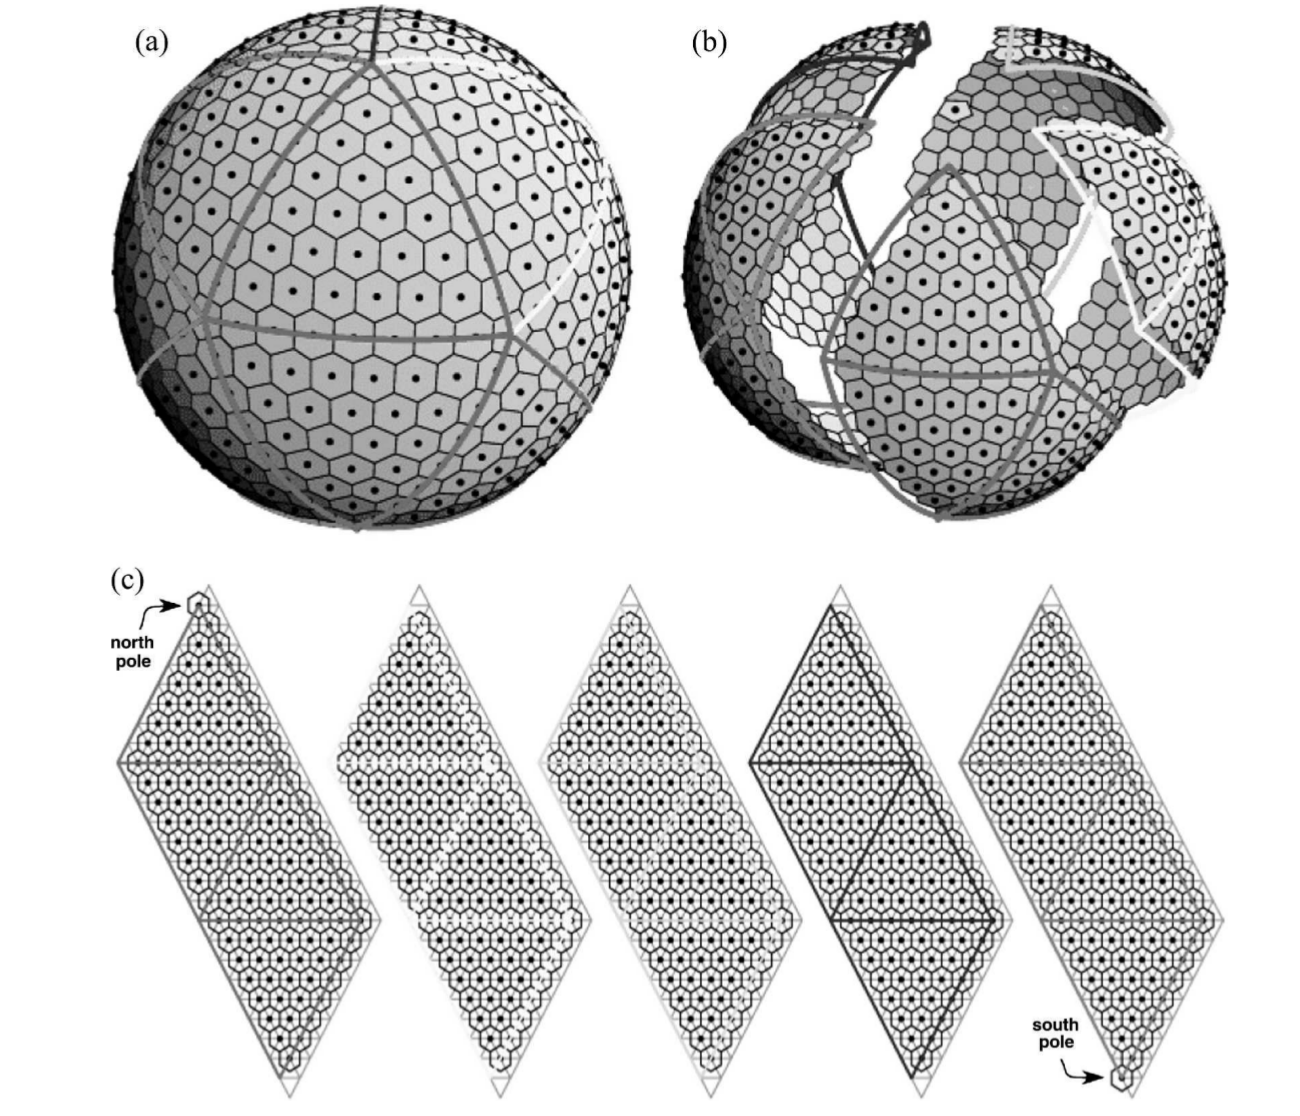
\includegraphics[width=\imsize]{figures/lipcomb}%
\caption{\label{fig:hexpent} The spherical hexagonal-pentagonal grid introduced by Lipscomb and Ringler \cite{lipscomb}}
\end{figure}

\subsection{Multidimensional Positive Definite Advection Transport Algorithm}
Smolarkiewicz' himself is also still active in the development of the Multidimensional Positive Definite Advection Transport Algorithm (MPDATA), a multi-dimensional generalization of the original approach by Smolarkiewicz described in this rapport \cite{mpdata}. This finite-difference method is still in wide use, and recently the transition to finite-volume has been made. MPDATA evolved and expanded over time; according to Smolarkiewicz (2005)
\begin{quotation}
[...] MPDATA evolved from an advection scheme into a class of generalized transport algorithms that expand beyond advective transport to alternate PDEs and complete fluid models with a wide range of underlying governing equations.
\end{quotation}

\clearpage
\subsection{Schemes without diffusion}
There are also schemes that have no diffusion. An example of such a scheme is a fully Lagrangian Advection Scheme. As opposed to an Eulerian fixed grid, Lagrangian schemes use a grid that moves with the flow. That means that the derivatives are calculated in the Lagrangian frame of reference since the advection equation can best be described in a Lagrangian frame. The two key components of a Lagrangian scheme are a method to follow the characteristics, and a method to view the solution on a Eulerian grid. There are two different kinds of Lagrangian schemes: in a fully Lagrangian scheme the grid is attached to, and moves with, the flow, and needs typically to be re-meshed after a finite number of steps, there are however also fully Lagrangian schemes that don't need to be re-meshed \cite{nodif}.

\section{Conclusion}
The advection equation is important in many areas of climate modeling. Because diffusion is a threat to reliable advection simulation, it is important to develop anti-diffusion techniques that are both efficient and accurate. Smolarkiewicz' iterative approach, later generalized into MPDATA, is such a technique; since it iterative in nature it is fairly straightforward to implement and in reasonable computation time it is as accurate as some of the more complex hybrid schemes.

The numerical results shown in this report show that with the right parameters even a simple technique such as the iterative approach by Smolarkiewicz works already quite well to reduce the diffusion.

For even more realistic and reliable results the existing techniques need still to be improved. Examples of some advanced grids that were introduced are the reduced grid \cite{spee} and the spherical hexagonal-pentagonal grid \cite{lipscomb}. MPDATA, the multi-dimensional generalization of Smolarkiewicz' scheme has also been expanded and improved to cover generalized transport algorithms and complete fluid models with a wide range of underlying governing equations. Fortunately there are also schemes, such as the fully Lagrangian schemes, that do not have diffusion at all.

Despite the existing efficient schemes it is still necessary to search for improvements to be able to model climate more accurately.

\bibliographystyle{plain}
\bibliography{report}

\end{document}
